\documentclass[oneside]{book}
\usepackage[a4paper, total={6in, 8in}]{geometry}
\usepackage[english]{babel}
\usepackage[utf8]{inputenc}
\usepackage[T1]{fontenc}
\usepackage{cancel}
\usepackage{amsmath}
\usepackage{amsfonts}
\usepackage{dsfont}
\usepackage{listings}
\usepackage{hyperref}
\usepackage{siunitx}
\usepackage{fancyhdr}
\usepackage{textcomp}
\usepackage{makecell}
\usepackage[font=small,labelfont=bf]{caption}
\usepackage{pdfpages}
\usepackage{multicol}
\usepackage[ruled,vlined]{algorithm2e}
\usepackage{soul}
\usepackage{mhchem}
\usepackage[toc, page]{appendix}
\usepackage{float}
\usepackage{wrapfig}
\usepackage{braket}
\usepackage{xcolor}
\usepackage{mathtools}
\usepackage{physics}
\usepackage{float}
\usepackage{subcaption}
\usepackage{tgbonum}


%Zotero Bibliography
%\usepackage{apacite}
%\addbibresource{bibliography.bib}


\pagestyle{fancy}
\fancyhf{}
\lhead{\rightmark}
\cfoot{\leftmark}
\rfoot{\thepage}

\setcounter{secnumdepth}{5}

\lstset{
    frame=tb, % draw a frame at the top and bottom of the code block
    tabsize=4, % tab space width
    showstringspaces=false, % don't mark spaces in strings
    numbers=none, % display line numbers on the left
    commentstyle=\color{green}, % comment color
    keywordstyle=\color{red}, % keyword color
    stringstyle=\color{blue}, % string color
    breaklines=true,
    postbreak=\mbox{\textcolor{green}{$\hookrightarrow$}\space}
}

\renewcommand{\lstlistingname}{}% Listing -> Algorithm
\renewcommand{\lstlistlistingname}{Algoritmi}% List of Listings -> List of Algorithms


\renewcommand*{\listalgorithmcfname}{}
\renewcommand*{\algorithmcfname}{}
\renewcommand*{\algorithmautorefname}{}
\renewcommand{\thealgocf}{}
\newcommand{\mathcolorbox}[2]{\colorbox{#1}{$\displaystyle #2$}}
%\renewcommand{\familydefault}{\rmdefault}


\title{\Huge\textbf{Computational microbial genomics}}

\author{
  Giacomo Fantoni \\
  \small telegram: \href{https://t.me/GiacomoFantoni}{@GiacomoFantoni} \\[3pt]
\small Github: \href{https://github.com/giacThePhantom/computational-microbial-genomics}{https://github.com/giacThePhantom/computationl-microbial-genomics}}

\begin{document}
\maketitle
\tableofcontents

\chapter{Introduction}

\section{Microbes}
Microbes are defined as whatever is not visible at the human eye: bacteria cells' dimensions are in the order of micrometre, while viruses in the order of nanometre.
It is obvious how there is no visible part by eye.
This is particularly true for viruses: their dimension make them almost impossible to perceive by any other method than genomics.

	\subsection{Prevalence of microbes}
	We are living in a microbial world: more than $90\%$ of the biomass is composed of them and they are responsible for a great part of the biochemical cycle.
	Microbes can thrive in a variety of environment and according to some estimates they compose $10^{17}g$ of biomass.
	To put that in context the overall weight of the human species is three or four order of magnitude less.
	They also form the human microbiome, with important medical implication.

	\subsection{Difficulties in studying them}
	Of the predicted $30$ million species to exist only thousands can be cultured in isolation in the lab.
	There is a need to create a way to directly study and characterized samples taken from the environment.

\section{Genomics}
Once the genetic material is isolated and sequenced a huge amount of information needs to be interpreted.

	\subsection{History of sequencing}

	\begin{multicols}{2}
		\begin{itemize}
			\item The first sequenced gene was one of a bacteriophage.
			\item Also the first complete genome wase one of a bacteriophage and is used by ILLUMINA as a control.
			\item The first bacterial genome was published in $1995$ and was that of Haemophilus influenzae.
				It has a dimension of $1.8Mb$ and sequencing took a year to complete.
			\item The first archea was sequenced in $1996$.
			\item In $1996$ the genome of S. cerevisiae has been sequenced and it was noticed that the genome shows a considerable amount of genetic redundancy.
		\end{itemize}
	\end{multicols}
	After having sequenced the genomes there is a need to elucidate the biological functions of the genes contained in them.

	\subsection{Comparative genomics}
	Studying two different strains of the same organism allows to link difference in the genome to difference in phenotype.

	\subsection{Metagenomics}
	Metagenomics is the study of the DNA from all the genomes in an environment.
	By sampling all of the DNA from a given environment, it is possible to study the presence of bacterial ecosystems, independent of the ability to culture each bacterial strain in the laboratory.
	Large evolutionary radiation of bacterial lineages whose members are mostly uncultivated and only known through metagenomics and single cell sequencing have been described as nanobacterial.
	They have small genomes and lack several biosynthetic pathways and ribosomal proteins.

\section{Leveraging computational power}
Despite the advantages in DNA sequencing technology the sequencing of genomes has not progressed beyond clones on the order of the size of $\lambda$ because of the lack of sufficient computational approaches that would enable the efficient assembly of a large number of independent, random sequences into a single assembly.
When moving from low-throughput to high-throughput biology statistical power is needed: the genome of a bacterium must comprise all the DNA coding molecules present in the cell.
With millions of reads from NGS of an environmental sample, it is possible to get a complete overview of any complex micro biome with thousands of species.

	\subsection{Comparing low-throughput and high-throughput pipeline}
	Let's consider the pipeline to find the pathogenic agent for a novel outbreak.
	In a low-throughput one a panel of reasonable putative causative agents is identified.
	Then one-by-one cultivation protocols to grow the agents from the infected tissue are performed.
	The pipeline ends when a pathogen grows in a sample.
	This is very time consuming.
	High-throughput instead sequences the full DNA repertoire of the sample and try to identify the pathogen by its genomic signature.

\graphicspath{{chapters/images/01/}}

\chapter{\emph{Escherichia Coli} general informations}
\section{\emph{E. coli} genomics}
\emph{Escherichia Coli} is a Gram-negative, facultative anaerobic, rodshaped, coliform bacterium, it pertains to the phylum of proteobacteria and to the family of Enterobacteriaceae. It can be grown easily and inexpensively. It has got genome with a length between 4.5 - 4.7 M bases, including about 4000-5000 genes, and about seven ribosomal RNA operons. Only the 38\% of the genes of K-12 (one of the most studied bacterial strains of \emph{E. coli}) were experimentally identified, overall 40-50\% of the genes are to date without a known function.
The original \emph{E. coli} strain K-12 was obtained from a stool sample of a
diphtheria patient in Palo Alto, CA in 1922.

\subsection{\emph{E. coli} long-term evolution experiment}
The \emph{E. coli} long-term evolution experiment led by Richard Lenski is one of the longest evolutionary experiments ever made (search "\textit{The Longest-Running Evolution Experiment}"). The experiment started on 24th February 1988, and since that moment 12 populations of \emph{E. coli} have been cultivated in the same environment. After each day (corresponding to the time of development of approximately 7 generations), a portion of bacteria from each flask was introduced in a new one, and let proliferating in it. Every 500 generation, it has been saved a sample of the bacteria of each flask, in order to track the evolutionary changes made. Today the experiment is on-going, and researchers reached approximately the 66000th generation. The study suggests a series of conclusions, to cyte "long-term adaptation to a fixed environment can be characterized by a rich and dynamic set of population genetic processes, in stark contrast to the evolutionary desert expected near a fitness optimum" (Good et al 2017). In fact, despite of the fixed environment, some bacteria developed the capacity to aerobically grow on citrate, which is unusual in \emph{E. coli} (around generation 31,000) and developed complex mutation patterns.


\subsection{\emph{E. coli} strains}
\emph{E. coli} could be found as commensal strains, pathogenic strains, or environmental strains. The pathogenic strains could pertein to these categories (which are not exclusive): enteropathogenic (EPEC), enteroinvasive (EIEC), enterotoxigenic (ETEC), diffusely adherent (DAEC), adherent invasive (AIEC), shiga-toxin producing (STEC), enteroaggregative(EAEC), extraintestinal pathogenic (ExPEC). Resistances to antibiotics make even more difficult the process of categorization of \emph{E. coli}.
In 2011 in Germany, an outbreak of Stx-EAEC was responsible of the death of some people. An efficient counter-measure was found by sequencing the genome of those bacteria.

Shigella is \emph{E. coli} with shiga toxin. It had been an issue for toxonomists.

Most of the genes are on plasmids, circular, additional to chromosome, and can be moved easily horizontally. Plasmids between different strains can be moved in enterobacteriacae, this doesn't happen normally in other families.
Some \emph{E. coli} strains are even capable of causing tumors in humans: for example, colibactin-positive \emph{\emph{E. coli}} can cause colon and rectal cancer, by creating mutations which are responsable of the of the cancer onset.

several antigens can be used by taxonomists to cathegorize \emph{E. coli} strains. In particular there are the O, H, K antigens, respectively related to the somatic, the flagella and the capsule. O antigens are 171, Ks are 80 and Hs are 56.

\subsection{PanPhlAn - strain detection and characterization}

Pangenome-based Phylogenomic Analysis (PanPhlAn) is a strain-level metagenomic profiling tool
for identifying the gene composition and in-vivo transcriptional activity of individual strains in metagenomic samples. PanPhlAn’s ability for strain-tracking and functional analysis of unknown pathogens makes it an efficient tool for culture-free infectious outbreak epidemiology and microbial population studies (\href{http://segatalab.cibio.unitn.it/tools/panphlan/}{PanPhlAn reference}). This tool was for example used to study the strain responsible of an outbreak in Germany in 2011. This strain was a shiga-toxigenic Escherichia coli (STEC), and the study was conducted by Loman and collegues in 2013.
This method outlasted the traditional one.


sequencing means generally to sequence everything, it's normally difficult where to find it, although in \emph{\emph{E. coli}} is quite easy to understand the provenience.
from all the world, populating diversity of \emph{\emph{E. coli}}, every time we sample we find points which are different from the reference genomes.
points overlapping are people living together and share bacterias


\subsection{Genomes of \emph{E. coli}}

In the genome of \emph{E. coli} strains, it is possible to distinguish:

\begin{itemize}
    \item \textbf{Core genome}: the set of all genes shared by all membrers of a bacterial species, it includes 1000 up to 3000 genes.
    \item \textbf{Accessory or dispensable genome}: the set of genes present in some but not all genomes within the same bacterial species. found on a single strain or in a subset of strains.
    \item \textbf{Pangenome}: core genome + accessory genome. set of all the genes foundable in the species strains. It is said to be \textit{\textbf{"closed"}} when pangenome size tends to a maximum as number of genomes increases, instead it is \textit{\textbf{"open"}} when pangenome keeps increasing as you add new genomes
\end{itemize}


Sequencing more organism of the same species means to lower the amount of genes in the core genome and augment the numer of those in the pan-genome (figure \ref{corepangenome}).
Because of technical problems the probability of getting a gene and not forget it is different from 0, so why probably the sequencing of other genomes would lead technically to a plummet to 0 of the pangenome. With some mathematical formulations we can predict a more probable plateau (Rasko David 2008).

% \begin{figure}[h]
% \caption{Core- and pan- genome of \emph{E. coli}}\label{corepangenome}
% \centering
% \includegraphics[width=0.6\textwidth]{EcoliCorePanGenome}
% \end{figure}


% \begin{figure}[h]
% \caption{It can be seen that 51\% of the genes are strain specific, and the other are shared between 2 to 20.  of \emph{E. coli}}
% \centering
% \includegraphics[width=0.6\textwidth]{genesSharedDifferentGenomes}
% \end{figure}


% \begin{figure}[h]
% \caption{A different definition of orthologous genes can modify the number of pan genes of a species. }
% \centering
% \includegraphics[width=0.6\textwidth]{orthologGenes}
% \end{figure}


% \begin{figure}[h]
% \caption{we predict a core genome size of 3079 genes for extraintestinal pathogenic \emph{E. coli}}
% \centering
% \includegraphics[width=0.6\textwidth]{coreGenomePredict}
% \end{figure}

each \emph{E. Coli} genome contains in a balanced way genes of the core genome and of the pan genome, for a total amount of genes correspondant to about 4700 genes (figure \ref{balancepancore}). Core genomes' genes are responsible of some basic cellular functionalities and utilities to survive environent, while instead elements of the pangenome are quite usually specific to the single strains, they are not always functionally well known.


% \begin{figure}[h]
% \caption{Balance between genes of the core- and of the pan-genome}\label{balancepancore}
% \centering
% 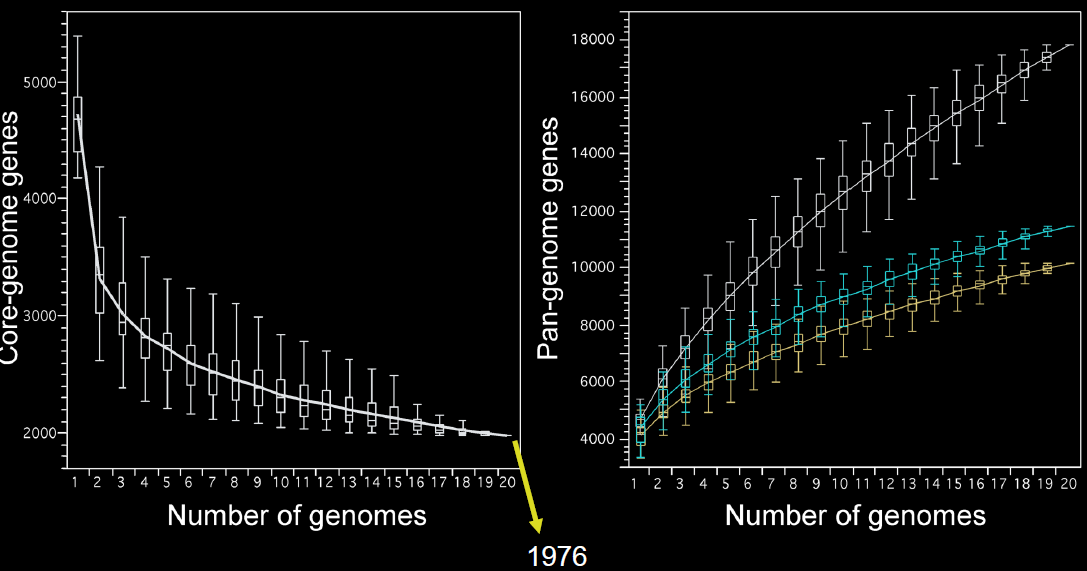
\includegraphics[width=8cm]{corePanGenEcoli}
% \end{figure}


ratios of the pan-genome and the core-genome are not equal in other
organisms behave differently.

\graphicspath{{chapters/images/03/}}

\chapter{NGS principles (second gen. sequencing) - From Sanger to third gen sequencing}

\begin{figure}[h]
\caption{}
\includegraphics[width=0.6\textwidth]{history-seq}
\label{discoveries-sequencing}
\end{figure}

NGS stands for \textbf{\textit{Next Generation Sequencing}}, and it represents the method of sequencing most used nowadays. Before that, a series of other discoveries were done, elencated in the figure \ref{discoveries-sequencing}.

\section{History of Sequencing}
\subsection{Progresses of sequencing}
As the time passes, the cost of sequencing the DNA is diminishing. The rate of decrease actually is higher than the one predicted by the \textbf{Moore's Law}, \textit{"Democratization of sequencing"} is seen nowadays, because of the costs lowering. After the Human genome project, several other animals and plants' genomes were sequenced.

\begin{figure}[h]
\caption{}
\centering
\includegraphics[width=0.6\textwidth]{sequencingCost}
\label{Moore's law graph}
\end{figure}

The methods of sequencing actually can be grouped in three \textbf{groups}, that are:

\begin{itemize}
	\item \textbf{Chemical degradation} of DNA: it includes the method of Maxam-Gilbert
	\item \textbf{Sequencing by synthesis (“SBS”)} which is the most common approach and the first to be developed. It uses DNA polymerases in primer extension reactions Illumina, Pacific Bioscences, Ion Torren and 454
	\item \textbf{Ligation-based}: sequencing using short probes that hybridize to the template, the technologies perteining to this class are SOLiD, Complete Genomics
	\item \textbf{Other:} Nanopores
\end{itemize}

\subsection{The Chain Terminators}

\begin{figure}[H]
    \centering
    \begin{subfigure}[b]{0.49\textwidth}
        \centering
        \includegraphics[width=\textwidth]{DNA-molecule}
        \caption{Normal DNA molecule, with oxydrilic group ligated to $3'$-ends}
        \label{normalDNAaddition}
    \end{subfigure}
    \hfill
    \begin{subfigure}[b]{0.49\textwidth}
        \centering
        \includegraphics[width=\textwidth]{chain-term}
        \caption{Figure representing the difference between a normal DNA chain and one with chain terminators}
        \label{ChainTerm}
    \end{subfigure}
    \caption{Normal DNA synthesys \textit{vs} Chain terminators}
\end{figure}


Normally, the addition of new nucleotides to a generated molecule of DNA happens with the $3'$-end of the nucleotide chain (figure \ref{normalDNAaddition}). Chain terminators are dideoxy nucleotides, ddNTPs, that cannot be further extended. These nucleotides aren't able to add a new nucleotide on the $3'$-end, as they have not the needed oxydrilic group (figure \ref{ChainTerm}).

\subsection{Sanger method: the first one}

\begin{figure}[h]
\caption{The \textit{Sanger}'s method process}
\centering
\includegraphics[width=\textwidth]{Sanger}
\label{Sanger}
\end{figure}

The first method ever used to sequence DNA was designed by Frederick Sanger. The Sanger manual sequencing system consists in an \textit{in vitro} process, which is described in figure \ref{Sanger}, also named as \textit{"primer extension"} method. It is performed over a single-filament DNA sample, and it uses the chain terminators nucleotides, a type for each nucleobase: ddATP, ddGTP, ddTTP, ddCTP.

The reaction is done inside four different reactions tubes, each containing the sample DNA to be reproduced, a DNA polymerase, the normal nucleotides and one of the four possible chain terminator. The chain terminators are marked with sulfur-35, a radioactive atom. In each tube, the corresponding dideoxy-nucleotide was used with a concentration 10 times lower than the other "normal" nucleotides.

From the polymerization reactions, several molecules of DNA were produced, with different length: each replicative cycle is in fact terminated after the addition of a chain terminator nucleotide.

To reconstruct the initial DNA sequence, a long PAGE gel was prepeared, with high concentration of urea ($6 - 7 M$) to avoid the coiling of the DNA single-filaments. To run the gel, high voltages were required and it had to be higly resolutive, as DNA's fragments are different only for a nucleotide. It was needed to do an auto-radiography of the gel in order to see the bands, in order to evidentiate the fosphorescent signals.

To read the sequence you have to start from the shortest fragments, at the end of the gel, and carefully go up along the gel, looking for the first presence of a band in one of the four runs. \\

\textbf{Past procedures: }In the past, the Klenow's fragment (part of the $1^{st}$ DNA polymerase) was used to perform the Sanger method, and the DNA to be sequenced was inserted inside the genome of an M13 phage.


\subsubsection{Automatic sequencing}
It does not use the radioactive signals, instead it uses fluorescent proteins. Several versions were developed after modifications of the Sanger method, in this order:

\begin{enumerate}
	\item fluorescent primers marked with a single fluorochrome.
	\item four aliquotes of the same primer were used marked with four different fluorochromes, able to emit different fluorescences.
	\item four different fluorochromes were used to mark the single ddNTPs
\end{enumerate}

Thanks to the use of 4 different fluorochromes, it was possible to use a single electrophoretic lane to carry the sequencing reaction. For this type of sequencing also, a cyclic replicative reaction was performed, with this procedure, made possible by using a thermal cycler:

\begin{enumerate}
	\item \textbf{Denaturation at $95$°C} of the DNA to be sequences
	\item \textbf{Annealing at $50-70$°C} of the primer specific to one of the two filaments
	\item \textbf{Extension at $72$°C} by using a \textit{Taq}-polymerase. The use of the Taq-polymerase makes it possible to avoid the formation of coiled structures in the DNA molecule to be sequenced.
\end{enumerate}

Traditionally, also in this type of sequencing it is used a long PAGE gel, as the Sanger's one, but with a great difference: all the ddNTPs are inserted in the same electrophoretic run, and after it, it is not needed an auto-radiography. Fluorescence, instead, can be triggered simply by irradiating the DNA molecules synthesyzed, which produce different fluorescences with different wavelengths.

\begin{figure}[h]
\caption{}
\centering
\includegraphics[width=0.8\textwidth]{automaticSang}
\label{}
\end{figure}


More usefully, this sequencing method is performed by using a capillar, filled with a synthetic polymer, with the same function of polyacrillamide.

At the end of the analysis, it is produced an electropherogram, with a color depicting the probability of each nytrogen base in each position. The production of the electropherogram is made better thanks to algorithms to boost signal/noise ratio, to correct the dye-effects, and other effects that generate systemic errors. %TODO dye-effects

\begin{figure}[h]
\caption{}
\centering
\includegraphics[width=0.8\textwidth]{elettroferogramma}
\label{}
\end{figure}

\begin{figure}[h]
\caption{The implementation of capillary sequencing machines gave the possiblity to make more runs than with the others. A $\tilde 1000$ fold productivity increase was allowed}
\centering
\includegraphics[width=0.8\textwidth]{progressSangerMachines}
\label{}
\end{figure}

Regarding the Sanger machines in use, the upgrades viewable in figure \ref{progressSangerMachines}. Based on the same technology, new machines were developed and it was obtained a $\tilde 1000$ fold improvement.
\\
When talking about the \textbf{human projec}t, it is important to specify that most of the job was done by using the Sanger automatic sequencing method.


\section{Development of Sequencing Machines}
The way you can get to the point could be different based on technology and the wanted output, comprised quality.

SOLID gave only $35$-$75$ sequenced bases, and it is not used anymore; Sanger sequencing, the capillary, can give up to 1000 read length, with a low output; on MINION it was possible to sequence an entire genome of \textit{E. coli}
A pletora of sequence machines are available today. None of the machines are able to sequence DNA from a sample of blood, some things have to be done. Nowadays \underline{machines producing bigger outputs of short reads are prefeared}.

\begin{figure}[H]
\caption{It can be noticed how recent developments had the scope of increasing the output data}
\centering
\includegraphics[width=1\textwidth]{sequencingMachines}
\label{}
\end{figure}

At the top of the market nowadays there are ILLUMINA machines, that use sequencing by synthesis method, NovaSeq is the biggest one. They need to amplify the signal through clusters formation.

\begin{figure}[H]
\caption{}
\centering
\includegraphics[width=0.8\textwidth]{sequencingMachinesIllumina}
\label{}
\end{figure}

\section{Next Generation Sequencing NGS}

The NGS protocol requires $3$ steps, that are:

\begin{enumerate}
	\item \textbf{Sample preparation}: series of fragments added
	\item \textbf{Clonal amplification}: which is is needed to replicate fragments attached to the solid surfaces, since machines are not sensible to single molecules
	\item \textbf{Sequencing}: ILLUMINA sequencing is one of the techniques used to obtain sequence data nowadays
\end{enumerate}

Tools pertaining to the $3^{rd}$ generation are those that permit to read a molecule without replicating it.

\subsection{Fragments/Library preparation}
Most of the sequences sequenced are fragmented in short read sequences, since most of the machines today used aren't able to sequence reads longer than some hundreds of nucleotides.

% Fragmantation is so required to generate shorter filaments from the sequences. In the case of mRNA (cDNA libraries) the fragmentation process is not needed, as the lengths are already short enough.

The fragments obtained have to be prepeared for the sequencing process, through a process called \textbf{tagmentation}. The obtained fragments are shown in the figure. Those fragments are provided with one or two indexes, called also barcodes, two sequencing primer binding sites and regions complementary to the oligonucleotides present in the chamber (see in Clonal amplification chapter). The fragments' length has to be checked, depending on the scope of the process. Indexes are needed to run sequencing process on multiple samples, they are needed to distinguish those; when they are two, they permit to distinguisch also the 2 types of sequencing that are performed, forward and reverse.

P5 and P7 are the oligos needed to attach fragments to ILLUMINA sequencing machines.

\begin{figure}[h]
\caption{Figure representing the a good prepeared fragment, it has two indexes, two sequencing primer binding sites and regions complementary to the oligonucleotides present in the chamber}
\centering
\includegraphics[width=0.8\textwidth]{tagmentedFragments}
\label{}
\end{figure}

%what is a good fragment? %TODO

\subsection{Clonal amplification and ILLUMINA sequencing procedure}

\begin{figure}[h]
\caption{}
\centering
\includegraphics[width=0.6\textwidth]{clusterAmplification}
\label{clusters}
\end{figure}

Clonal amplification are necessary to amplify the signal from each single fragment.
ILLUMINA machines make use of clusters to sequence DNA. Clusters are a group of DNA
strands positioned closely together and generated from a single DNA filament. Generally, Each cluster represents thousands of copies of the same DNA strand in a 1–2 micron spot (figure \ref{clusters}).

\begin{figure}[h]
\caption{}
\centering
\includegraphics[width=0.8\textwidth]{rigidGeneration}
\label{rigid}
\end{figure}

On patterned flow cells, the clusters' formation location could be known or not, in the first case it is said that there is a "Rigid registration" (figure \ref{rigid}).\\


ILLUMINA sequencers normally use slides of glass, named flow cells, and the fragments to be sequenced are able to flow over the channels. The temperature inside the cells can be changed to produce ligations or separations. The surface of the cells is functionalized with a series of oligos complementary to library adapters.

Two kids of flow cells, the \textit{patterned} flow cell permits to create clusters in specific positions, inside nanowalls, contrarily to \textit{Random Flow Cell} which instead have randomly positioned clusters.
\begin{figure}[h]
\caption{}
\centering
\includegraphics[width=0.6\textwidth]{randomPatternCells}
\label{}
\end{figure}
\\

Once the fragments are made flow over the chambers, they can bind only to p5 or p7 (ILLUMINA oligos), the two oligos functionalizing the plate. Once the fragments are attached to the surface, using temperature and solvents flows you can control the sequencing process. To see the entire procedure:
(procedure on Youtube: \href{https://www.youtube.com/watch?v=womKfikWlxM}{video about ILLUMINA sequencing}). In the video, it is shown the two index sequencing process.
\\
\\


\begin{figure}[H]
    \centering

    \begin{subfigure}[b]{0.39\textwidth}
        \centering
        \includegraphics[width=\textwidth]{singleIndex}
        \caption{single index}
    \end{subfigure}
    \hfill
    \begin{subfigure}[b]{0.60\textwidth}
        \centering
        \includegraphics[width=\textwidth]{doubleIndex}
        \caption{double index}
    \end{subfigure}
    \caption{Single/double index for ILLUMINA sequencing}
    \label{singDoubInd}
\end{figure}

With 1 and 2 indexes the sequencing process actually differs, as shown in figure \ref{singDoubInd}


\begin{figure}[H]
\caption{}
\centering
\includegraphics[width=0.7\textwidth]{ILLUMINArev}
\label{ILLUMINArev}
\end{figure}

To perform the sequencing process, ILLUMINA machines utilize \textit{reversible terminators} (figure \ref{ILLUMINArev}). They permit a real time analysis of the sequencing by synthesys reaction, and because of this they are different from the Sanger method. Fluorophores are reversible, they can be cleaved to eliminate the light signal.

\begin{figure}[h]
\caption{}
\centering
\includegraphics[width=0.8\textwidth]{ChannelILLUMINA}
\label{ChannelILLUMINA}
\end{figure}

To perform their activity, ILLUMINA sequencers could be of 3 different types: 4-Channel, 2-Channel or 1-Channel, depending on the number of fluorescent molecules used. In the case of the 4-Channel technology, 4 images are taken in each cycle, and each  cluster appears in only one of four images \ref{ChannelILLUMINA}. 2-Channel technique is used by some sequencing machines, like NextSeq 550, MiniSeq, NovaSeq 6000\\

4-Colors base calling
is needed to to make
the true signal the purest, and after, The base with the highest intensity becomes the called base for that cluster. In the case no base is clearly related to a position, \textit{N} is the result.


The reading process could be done in two ways: through single reads, on a single extreme of the fragments, of paired-end, on both the extremes. The second one in particular gives structural and 2 sequence  informations.


\subsection{Pacific Bioscience (PacBio)}
the long DNA filement to be sequenced is attached to a polymerase, over the surface of a SMRT (Single Molecule Real Time) cell. This cell is really small, and at each nucleation process a light signal is emitted. The produced light is not able to get out of the walls, and its duration is extremely restricted. Sequencing, also in this case, is made by sequencing, and the main advantage consists in the possiblity of sequencing really big DNA molecules.\\
In the video \href{https://www.youtube.com/watch?v=_lD8JyAbwEo}{PacBio procedure} it is briefly shown how the process works and what are the strategies used to reduce errors.

\begin{figure}[h]
\caption{}
\centering
\includegraphics[width=1\textwidth]{PacBIO}
\label{}
\end{figure}


\subsection{Nanopore sequencing}
Intramembrane proteins are used, sequence detected through the passage of DNA nucleotides, which produce different voltage changes. During the first periods, this type of instruments gave great amount of errors, nowadays the technique is improving.
\href{https://www.youtube.com/watch?v=E9-Rm5AoZGw}{Nanopore Sequencing}

\graphicspath{{chapters/images/04/}}
\chapter{Sequencing data}

\section{Choosing the optimal technology}
When performing a genetics or genomics study it is best to be as hypothesis driven as possible and use already available data to guide the new analysis.
Moreover to choose the optimal sequencer the parameters that need to be considered are:

\begin{multicols}{2}
	\begin{itemize}
		\item Throughput.
		\item Cost.
		\item Read lengths.
		\item Data output (reads per run).
		\item Coverage.
		\item Sequencing errors (indel, substitution, CG deletion, AT bias).
		\item Library preparation compatibility.
		\item Speed (run time).
	\end{itemize}
\end{multicols}

	\subsection{Comparing different sequencing technologies}

	\begin{multicols}{2}
		\begin{description}
			\item[Illumina NovaSeq]: optimal for sequencing a lot of DNA molecules at the same time like in the case of genomes or metagenomes.
				It can’t go over $300 bp$ readlines run, but it has the highest throughput so far.
				It is capable of multiplexing, differentiating the different samples with an unique barcode.
			\item[Illumina iSeq]: optimal for sequencing shorter genomes.
			\item[NanoPore (minion)]: it is a pocket-sized wet-lab free sequencer for DNA, RNA and (possibly) proteins, but the read lengths is smaller than Illumina's.
				The machine is cheap;, but the running flow is more expensive over time.
				It's a real-time sequencer.
			\item[PacBio]: has very long reads but carries a high amount of error.
		\end{description}
	\end{multicols}

	A solution to reduce the impact of error or weaknesses of one of the sequencers is to use more than one for the same project.
	Consider there is a need to sequence the genome of a bacterium: PachBio would give a lot of sequence errors, while Illumina wuild be unable to reconstruct the sample due to assembly ambiguities.
	In the end PacBio will construct the genome and Illumina will correct sequence errors.
	This solution doesn't work in complex sample with more than one genome, because there is no way to a priori which reads are coming from one organism.
	Another widely adopted solution is to sequence multiple times one molecule so to reduce random errors.
	This is effective but does not resolve systematic error like the one of PacBio with homopolymers.

	\subsection{Sequencers' output}
	All sequencing platforms translate the physical read signal into files in FASTQ format.
	This files contain the sequencing reads and the quality of each base.

\section{Base callers}
A base caller is an algorithm that translates the analogical signal of the reading into numbers and nucleotides.
The most popular algorithm is Phred.
Phred tries to correct errors derived from the sequencing reaction and electrophoresis.
It was tested on a huge dataset of gold standard sequences (finished human and C. elegans sequences generated by highly-redundant sequencing).
Its results were compared with the traditional ABI base caller and Phred was considerably more accurate with $40$-$50\%$ fewer errors.
This algorithm need to be able to understand when it is impossible to recover an high quality sequencing and so it needs to be able to give up for low-quality reads.
The confidence that the base caller has to call a certain nucleotide ATCG is annotated in the FASTQ file, allowing for quality control downstream.

	\subsection{Errors solved by Ilumina's base caller}

	\begin{multicols}{2}
		\begin{description}
			\item[Phasing noise $\phi$]: when a certain base is not seen frequently, the first time in which it will reappear there will be a spike in the graph, increasing the signal of the nearby bases.
				This will cause errors in estimating the real nucleotide that is occurring in the site.
				This problem can be solved by waiting more time between readings, but the sequencing will be less efficient and the throughput will be lower.
				The machine needs to find a trade-off between efficiency and clear reading.
			\item[Signal decay $\delta$]: after a while the sequencer has read the same base, or the same repeated couple of bases, the signal will go down and at some point will be indistinguishable.
				At some point you will need to cut the read since it will be not trustable after a while.
			\item[Mixed cluster $\mu$]: two different fragments can enter the same cluster and the sequencer will read the two signals simultaneously.
			\item[Boundary effects $\omega$]:  in this case the machine needs to interpret an image and it cannot distinguish between the signal and the background.
			\item[Cross-talk $\mathcal{X}$]
			\item[Fluophore accumulation $\tau$]
		\end{description}
	\end{multicols}

	\subsection{Density on the flow cell}
	The density of the flow cell is the number of cluster in it.
	Under clustering will reduce the sequencer throughput, while over clustering will cause errors due to the limited resolution of the reading of the bases.
	There is a need to find the optimal number of cluster that maximises the throughput without introducing overlapping in the reading of clusters.

	\subsection{An ecology of base callers}
	Base callers need to find a satisfying trade-off between accuracy and computational efficiency.
	The quality is the estimation of the probability that the nucleotide in a certain position is correct.
	The PHRED score reported by the base caller and the PHRED score of mapping to a reference sequence are different.
	Base callers need to be calibrated with a standard to make sure that the estimation of the quality is accurate enough.

\section{FASTQ format}

	\subsection{Composition}
	The FASTQ format is composed by:

	\begin{multicols}{2}
		\begin{enumerate}
			\item ‘@’ followed by a sequence identifier.
				This identifier contains the unique instrument name, the flowcell and tile number, the x and y coordinates of the cluster within the tile, the index number for multiplexing and the pair number of paired-end sequencing.
				In Illumina MiSeq, each flowcell has 8 microfluidic channels (lanes), each lane contains three columns with 96 tiles, and can sequence up to 96 multiplexed samples.
			\item The sequence. It could be mate paired for paired end sequencing.
			\item ‘+’, optionally followed by a sequence Identifier.
			\item The quality scores.
				Quality is a number based on the estimated probability of error.
				$p$=probability  of error, $Q = -10 \dot p$ .
				A base quality of at least $20$ is needed to reach  $1\%$ of error.
				A base quality of $40$ means the probability of error is $0.01\%$.
				The FASTQ quality score is the phred score +33, converted in CHAR code.
		\end{enumerate}
	\end{multicols}

	The FASTA file format is a FASTQ fomrat without the quality score reported and the seq ID is preceded by '>'.

	\subsection{Quality control: read length distribution}
	Quality scores are typically used to perform quality control and cleaning of the reads.
	This result in a FASTA output file to be used downstream.
	However there are algorithms that can use directly FASTQ files, performing autonomously the cleaning and quality control of the reads.
	The quality score is an indication of how well the sequencing run went.
	Typically the quality decreases when the read length increases due to the fact that sequencers have problem when are run in continuum.
	A solution to this problem is to cut the reads when the quality becomes too low.
	Another problem happens when the adapter is included into the read.
	This happens typically with short reads and a solution is to cut it and a part of the sequence.
	FastQC can be used to plot the quality distribution of the data.
	Another way to asses read quality is to consider the average quality of the entire read, discarding the low-quality ones.


	\subsection{Duplication artifacts}
	It is not frequent to see duplication, but it can be a problem especially when there is a need to quantify gene expression or copy number of genes in a bacterial genome.
	The distribution of the duplicates should be the same of the distribution of the reads.
	There should’t be any bias along the length of the reads, but if there is it should be due to a repetition of sequencing of the same read or when the adapter and primer have been read.

	\subsection{GC content analysis}
	Each organism has a signature GC content, so when plotting it a normal distribution is expected.
	Multiple peaks are an indicator of the presence of two different organisms.

	\subsection{K-mers frequency plot}
	K-mer frequencies are a way to catch systematic sequencing error: when mapping a genome it is now the relative frequency of each K-mer.
	That can be compared with the K-mers frequencies to catch systematic errors in sequencing and to assess its quality.
	Frequent k-mers can be a signature, as the GC content.
	The expected coverage of a k-mer with reads of length L:

	$$L_{cov} = \frac{L-k+1}{L} \, \times \, Cov$$

	Then, given a k-mer, it can be seen in how many reads it is present.
	For a typical K-mer its coverage should be around $40\%$.
	Coverage higher than $80\%$ should indicate that this k-mer is located in more than one position.
	Other values arises from errors.

	\subsection{Low-complexity artefacts}
	Same nucleotide repeats (especially A) are in a lot of cases artefacts.
	This is due to systematic error and can be evidenced through quality control.
	To measure if these sequence are in fact artefacts parameters to take into consideration are:

	\begin{multicols}{2}
		\begin{itemize}
			\item Low complexity.
			\item Low entropy.
			\item High compression (the artefacts increase the information inside the file).
		\end{itemize}
	\end{multicols}

	But some low-complexity sequences are not artefacts:

	\begin{multicols}{2}
		\begin{itemize}
			\item Hydrophobic transmembrane alpha-helical sequences in membrane proteins.
			\item CAG repeats in genes causing Huntington disease, spinal and bulbar muscular atrophy, dentatorubropallidoluysian atrophy.
			\item Proline-rich regions in proteins.
			\item Poly-A tails in nucleotide sequence.
			\item Micro-satellites.
		\end{itemize}
	\end{multicols}

	\subsection{FASTQ quality control (QC)}
	FASTQ quality control is the first step in any NGS pipeline.
	It consists of:

	\begin{multicols}{2}
		\begin{description}
			\item[Clipping/trimming]: removing (low quality) parts of reads.
			\item[Masking]: avoiding to consider parts of reads that can have low entropy for example.
			\item[Read removal]: discard low quality reads or reads that are too short after clipping.
		\end{description}
	\end{multicols}

	Additional features that can be exploited for QC are the GC content, clustering for contamination detection, TAG identification,ambiguous bases.

\graphicspath{{chapters/images/05/}}
\chapter{Mapping}

Mapping (or aligning) and assembly are the operations that allow us to make some sense out of fragments (input data) deriving from sequencing, produce assemblies. 

\begin{itemize}
    \item \textbf{Mapping} is a key step in a modern genomic analysis and consists in the process of aligning the reads on a reference genome, in order to assign them to a specific location. With mapping, insights like the expression level of genes can be gained.
    \item \textbf{Assembly} by contrast, is the process of aligning and merging overlapping sequences in longer consensus sequences in order to reconstruct the original sequence/genome.
\end{itemize}

A consensus sequence is  the calculated order of most frequent residues, either nucleotide or amino acid, found at each position in a sequence alignment
In many cases, someone may have already assembled the genome or part of the genome (available reference sequences), so we don't need to do sequence assembly, only mapping (like for the human genome). Assembly will be needed however when studying new organisms. 

Problems related to mapping and assembly: 

\begin{itemize}
    \item absence of DNA fragments covering the gaps, makes it difficult to order the contigs (since there is no connection)
    \item presence of DNA artefacts (those must be discriminated with Quality Control)
    \item repeated sequences
\end{itemize}

\section{Mapping}

The coverage, or read depth, is the average number of reads representing a given nucleotide in the reconstructed sequence (Some points of the reference sequence will be aligned with more reads, some with less. The average number of reads for each nucleotide is the coverage). 
The coverage of a genome is defined as the average coverage of each single nucleotide across all nucleotides of the genome. 
%Additional info and examples at:  https://thesequencingcenter.com/knowledge-base/coverage/#:~:text=Coverage%20is%20defined%20as%20the,reference%20genome%20Escherichia%20coli%20BW2952.
A coverage of 1x does not mean that all reads are read once. This would be true if sampling were systematic, but sampling is not systematic, it is random and is biased. Hence, a coverage of 1x means that on average each nucleotide is covered once, but there will be some nucleotides covered more and some not covered (0 coverage). 
The coverage can be represented with a coverage map and can also be defined theoretically as:

\begin{center}
    Pval = K e\textsuperscript{-lambda S} = Evalue/mn
\end{center}

where G is the length of the genome; N is the  number of reads; L is the average read length.
Knowing the wanted coverage is important to set up the machine in order to obtain the right number of reads (to achieve a certain coverage). A higher coverage means indeed more reads to be obtained. 

\subsubsection{Exercise on coverage}

\emph{How many reads do I need to cover the entire genome?}
Define the probability  to cover the full genome (with a certain epsilon subtracted - so not 100$\%$) or: define the number of reads N to cover the whole genome with a certain probability P = 1- epsilon.

\begin{figure}[h]
\centering
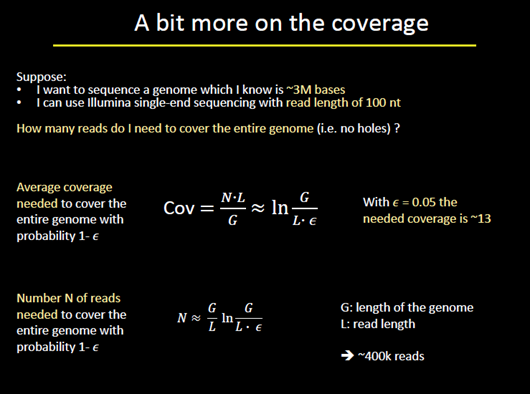
\includegraphics[width=0.6\textwidth]{coverage.png}
\caption{}
\end{figure}

In general, the sequence mapping process consists in performing comparisons between experimental sequence data (reads obtained with sequencing) with some reference information, like reference genomes and known genes (eg. the human genome). The comparison can lead to obtaining new information, such as the presence of SNPs which can be linked to pathological conditions or whatsoever, based on the starting point.

\begin{figure}[h]
\centering
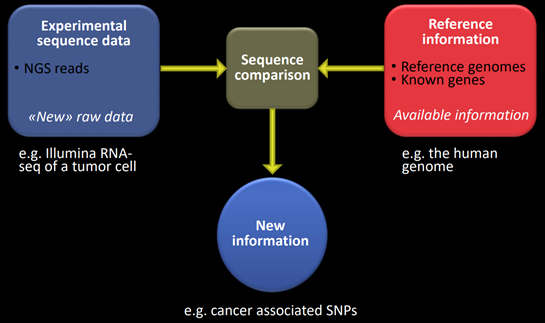
\includegraphics[width=0.6\textwidth]{SequenceComparison.png}
\caption{}
\end{figure}

\section{Mapping algorithm}

Over time many different mapping algorithms were implemented; some of them are not used anymore, while others are the base of current mapping and aligning genomic tools. 
Ideally, the \textbf{simplest aligning algorithm} could consists in:  
We have a smaller sequence that we want to align to a longer one. Start from the first position, align the query sequence against the subject, and look at how many nucleotides are correct (score: 4/10 = 40$\%$), then repeat for all positions until a perfect match is found (if found). The problem with this algorithm is that it doesn't consider insertions and deletions.

\subsection{Local vs Global alignment}
Sequence alignment can follow two different approaches.

\begin{enumerate}
    \item In \textbf{global alignment} an attempt is made to align completely the 2 sequences (end to end alignment). So global alignment finds the best alignment across the whole two sequences. This approach is suitable for comparing closely related sequences like homologous genes. 
    \item \textbf{Local alignment}, on the other hand, focuses on finding regions of similarity in parts of the sequences (so it aligns subsequences of the query sequence to a subsequence of the target sequence). This approach is suitable for aligning more divergent sequences or distantly related sequences. Used for example for finding out conserved patterns in DNA sequences of motifs in two proteins.
\end{enumerate}

Sequence similarity is connected with \textbf{evolutionary distance} (also for cell populations in a tumour). Very high similarity implies a very low distance. But when the similarity goes down and reaches the twilight zone, it is more difficult to define the evolutionary distance and to give meaning to results (the zone depends on the experiments).

\begin{figure}[h]
\centering
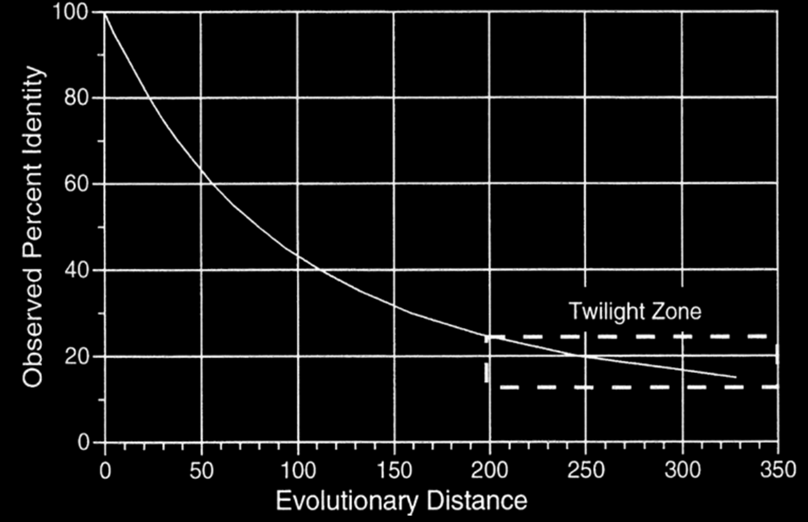
\includegraphics[width=0.6\textwidth]{EvolutionaryDistance.png}
\caption{}
\end{figure}

\subsection{Smith-Waterman algorithm  (local alignment) - 1981}

%Paper link: https://www.sciencedirect.com/science/article/abs/pii/0022283681900875?via%3Dihub
Take the algorithm for string recognition and apply it to find common molecular sequences. Not good for indels and substitutions. 
The S-W Algorithm is a local-alignment algorithm based on dynamic programming, whose aim is to find the best match among all possible (optimal local alignment) with respect to the scoring system used .
Firstly, we need to define a \textbf{score} for matches and penalties for mismatches and gaps (defined by the formula). 
The algorithm starts by putting zeros in the first row/column (\textbf{INITIALIZATION}). Then, starting from the first position H(1,1), at each iteration a number, based on the formula, is added (\textbf{ITERATION}). The number to be added is the greater between the 4 numbers defined by the formula, where d represents the penalty for gaps, and  s(x,y) = score when 2 NTs are the same (This gives a score of 5 if the 2 bases are equal, -3 if they are different) (PARAMETER SETTING).

\begin{figure}[h]
\centering
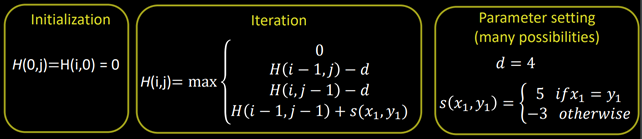
\includegraphics[width=0.6\textwidth]{Waterman.png}
\caption{}
\end{figure}

\textbf{Example}

First position H(1,1) = (G,C), max between: 

\begin{itemize}
    \item 0
    \item H(i-1, j) = 0-4 = -4
    \item H(i, j-1) = 0-4 = -4
    \item H(diag) + s(x, y) = 0 – 3 = -3
    \item $\xrightarrow[]{}$ We put 0
\end{itemize}

Second position H(2,1) = (A, G):

\begin{itemize}
    \item - 0
    \item -4
    \item -4
    \item -3
    \item $\xrightarrow[]{}$ We put 0
\end{itemize}

Third position H(3,1) = (C e C):

\begin{itemize}
    \item - 0
    \item -4
    \item -4
    \item 0 + 5 (since C=C)
    \item $\xrightarrow[]{}$ We put 5 
\end{itemize}

Here we also put an arrow indicating the nucleotide in the diagonal, to indicate that the 5 score derived from that point (hence from that path).  The arrows are needed to reconstruct the alignment at the end of the process. The iteration is performed for each cell of the table (column wise).
The parameters chosen for d (gap penalty) and s(x,y) (match or mismatch) can change the results. 
Final Solution: 

\begin{figure}[h]
\centering
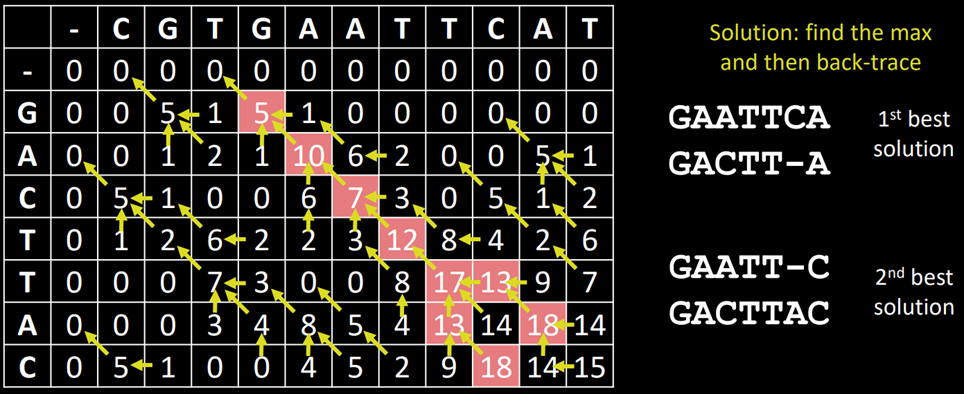
\includegraphics[width=0.6\textwidth]{Aligning.png}
\caption{Aligning CGTGAATTCAT and GACTTAC}
\end{figure}

Find the \textbf{maximum number} (18, here we have 2 of them) and go back following the arrows. In case of multiple highest scores, traceback should be done starting with each highest score.
From this path, the sequence is constructed by these rules:

\begin{itemize}
    \item A diagonal arrow represents a match or mismatch, so the letter of the column and the letter of the row of the origin cell will align.
    \item A horizontal or vertical arrow represents an indel. Vertical arrows will align a gap ("-") to the letter of the row (the "side" sequence), horizontal arrows will align a gap to the letter of the column (the "top" sequence).
    \item If there are multiple arrows to choose from, they represent a branching of the alignments. If two or more branches all belong to paths from the bottom right to the top left cell, they are equally viable alignments. In this case, note the paths as separate alignment candidates.
\end{itemize}

This algorithm is not used anymore due to a too high computational expense (huge number of comparisons for real genomes) and storage (memory and speed). In fact comparing two Eukaryotic genomes will result in a excessively great aligning matrix ($\sim$3Gb x $\sim$3Gb), and also using small reads against the human genome is unfeasible: 100 x $\sim$3Gb for each read!

\subsection{Needleman-Wunsch algorithm (global alignment)}

This global alignment algorithm was developed in 1970 and is also based on dynamic programming. The purpose of the algorithm is to find all possible alignments having the highest score. Again, a scoring system must be defined, then the algorithm proceeds in a similar way as the SW. 

\begin{figure}[h]
\centering
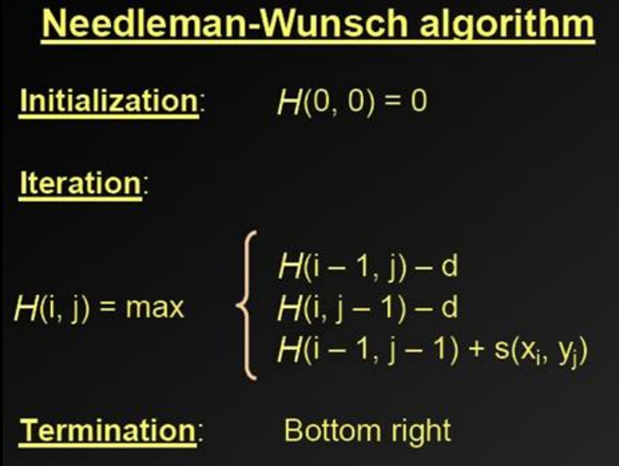
\includegraphics[width=0.6\textwidth]{Needleman.png}
\caption{}
\end{figure}

The differences are:

\begin{itemize}
    \item Initialization: we start from only one value, one zero, putted in H(0,0) (need to start from the first nucleotide - global). 
    \item The formula contains no 0 anymore, it adds the maximum score between 3 possible scores, we are always comparing with the first nucleotide of the sequence. 
\end{itemize}

\begin{figure}[h]
\centering
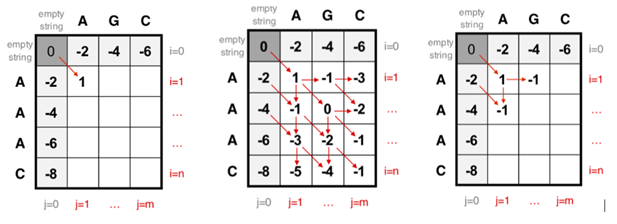
\includegraphics[width=0.6\textwidth]{Needleman2.png}
\caption{}
\end{figure}

New algorithms were implemented later. 
BWA and BowTie2 are the best ones available right now for short reads. Blast could go too but it would take a lot of time. 

\begin{figure}[h]
\centering
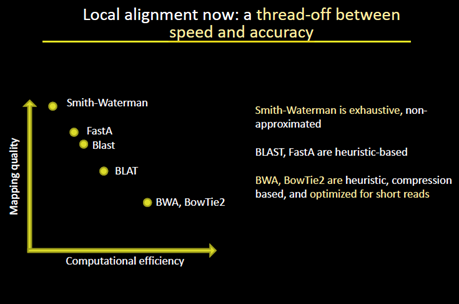
\includegraphics[width=0.6\textwidth]{LocalAlignment.png}
\caption{}
\end{figure}

The methods going from FastA to BowTie2 are \textbf{heuristic methods}: the solution found does not need to be the best one, but the best approximation given certain parameters (like time). Also, Blast gives an answer based on a fixed level of sequence similarity (in a reasonable amount of time) and gives no result under that level. So Blast online is not very sensitive, it is trained to provide only very good results to not overload the servers. 
A \textbf{heuristic}, or heuristic technique, is any approach to problem solving or self-discovery that employs a practical method that is not guaranteed to be optimal, perfect, or rational, but is nevertheless sufficient for reaching an immediate, short-term goal or approximation. Where finding an optimal solution is impossible or impractical, heuristic methods can be used to speed up the process of finding a satisfactory solution. Heuristics can be mental shortcuts that ease the cognitive load of making a decision.
BWA and BowTie2 are also ‘compression based’ algorithms, meaning that they exploit data compression techniques in order to compress reference genome files to reduce the number of bits used to encode the document (better explained below).

\subsection{BLAST (Basic Local Alignment Search Tool)}

%Tutorial: https://www.youtube.com/watch?v=HXEpBnUbAMo&ab_channel=JHUAdvancedAcademicPrograms
Despite its limitations, Blast is still used a lot and when it was first released it revolutionised the field making sequence alignment available for anyone and for any computer (it can be run online).
How does it work? Steps:

\begin{enumerate}
    \item \textbf{Seeding}: find perfect or almost exact k-mer matches (series of sequences with defined length). The idea is to look for identical short matches and try to expand from that. 
    \item \textbf{Extension}: extend the seeds at point one 1 with possibly some non-exact but high-score matches, that permit to obtain better alignments.
    \item \textbf{Evaluation}: create alignments for the regions of high-scoring extended seeds. Every time the statistical significance of the match is evaluated with methods inspired on the NW and SW approaches.  
\end{enumerate}

In online Blast tools the seed is set to 25/29. If a sequence of that length does not match perfectly another sequence we will have no results. One solution would be to lower the seed, but this cannot be done online because it would take too much time. Another option is to reduce the dataset in which we search.
There are many types of blast available, shown in figure:

\begin{figure}[h]
\centering
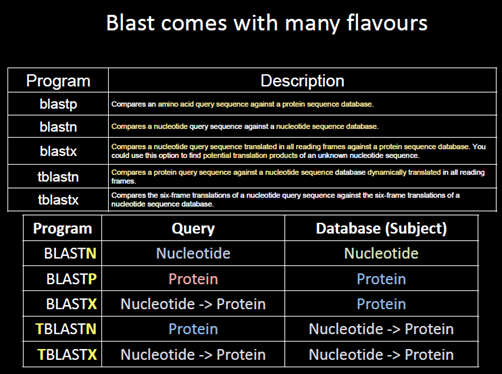
\includegraphics[width=0.6\textwidth]{Blast.png}
\caption{}
\end{figure}

\textbf{Scoring matrices} are very important especially for amino acids, they are used to score alignments between protein sequences. Blosum 62 (BLOcks SUbstitution Matrix) is one of the most used.
They put non simple penalties in substitutions of different amino acids, for example based on the functional properties of the substitutions. A scoring matrix contains values proportional to the probability that amino acid i mutates into amino acid j for all pairs of amino acids. Such matrices are constructed by assembling a large and diverse sample of verified pairwise alignments of protein sequences.
Other \textbf{parameters} can be set in online BLAST:

\begin{itemize}
    \item Max target sequences $\xrightarrow[]{}$ number of reported sequences 
    \item Expected threshold $\xrightarrow[]{}$ e-value
    \item Words size $\xrightarrow[]{}$ seed
    \item Gap cost $\xrightarrow[]{}$ cost for adding multiple gaps. Linear = twice the gap penalty (if I have to add a second gap after another one).
    \item Filter low complexity regions to avoid getting stuck 
\end{itemize}

\subsubsection{BLAST E-value}

If we have a match and the database is random, how many other matches I will likely find?

\begin{figure}[h]
\centering
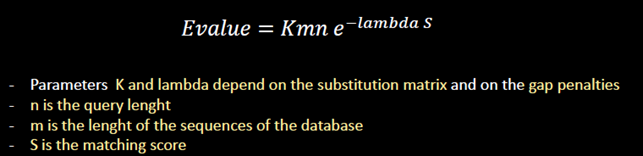
\includegraphics[width=0.6\textwidth]{Evalue.png}
\caption{}
\end{figure}

The \emph{e-value} represents the number of distinct alignments with a score equivalent to or higher than S, that are expected to occur in a database search by chance. An e-value of 10 means that up to 10 alignmentscan be expected to be found just by chance, given the same size of a random database. E-value can be used as a first quality filter for the BLAST search result, to obtain only results equal to or better than the number given by the e-value option. Blast results are sorted by E-value by default (best hit in first line).
The smaller the e-value, the better is the match. A small e-value means a low number of hits, but of high quality, whereas a high e-value indicates many hits, partly of low quality (if the number of better possible alignments is high, it means that it is particularly probable to find by chance an alignment which is better the the one found, and so it is more probable that those alignments are bad). 
There is a relationship between the E-value and the p-value. 

\begin{itemize}
    \item The E-value is the number of sequences that we would find by chance;
    \item The p-value measures the probability of finding by chance another sequence with an equal or better score.
\end{itemize}

\begin{center}
    Pval = K e\textsuperscript{-lambda S} = Evalue/mn
\end{center}

\subsection{Speed seed alignment}

There are algorithms implemented 10/15 years ago that focus on seeds -> not used anymore. 
Those methods cut both the reads and the reference sequence (read-sized pieces of reference sequence) into small seeds. The reference seeds are then stored in an index (hash look-up table).
The idea is to do that for all possible k-mers. Eg. we choose a seed of 10: the first starts at position 1, the second at position 2, ecc. And then to look up seeds for each read and identify the positions in genome where spaced seed pair is found. 

\begin{itemize}
    \item 1 SNPs means that at most 1 seed is not-matching.
    \item X SNPs means that at most X seeds are not-matching.
\end{itemize}

Algorithms based on this approach are: Maq, SOAP, MOSAIK. 
Problem: the lookup table (the reference) for the human genome is too big: 50Gb $\xrightarrow[]{}$ problem in RAM.

\subsection{Burrow-Wheeler alignment}
This algorithm is based on a very efficient way to store the reference genome, based on the BW transformation, that allows to have a reference index which is way lighter (with respect to the spaced seed approach); in fact, at the end of the transformations, equal letters are next to each other. It is successful because the database is compressed and does not need to be decompressed. However, when we compress a file, the compression must be reversible. There must be a way to go from the BW compressed/transformed index to the original one, to find reads in the genome. 
The search is based on finding suffixes of the reads in the BW structure. With this approach the index of the human genome is around 2GB. The algorithms BW-based are the fastest currently available. 
BWT is also used in text compression.
Example:
We want to compress the word BANANA
\begin{itemize}
    \item - we take all the rotations of the word
    \item we sort them based on lexigographic order (Lex order - lexicographical order is a generalization of the alphabetical order of the dictionaries to sequences of ordered symbols) 
    \item we take the last column
\end{itemize}

We end up with a string which is more compressible, there are sequences of the same letters that can be described at a higher level (Eg. there is 1 B, 2 NN, ecc)
In the method shown, in order to \textbf{reverse the transformation} and go back to the original word, the input sequence (output of the compression) is added as a column and then sorted (based in lex order), and this two passages are repeated as many times as are the characters of the sequence (8 in this case), obtaining at the end a matrix with equal number of columns and rows. As a result we go back to the ordered sequence of the word's rotations, in which the last one (last line) is the original input string. 
It takes a lot of time but it makes it reversible; plus, there are actually smarter ways to go back, such as ones base on the LF property.

\subsection{LF (Last-First) property}

As in the previous method, the first step consists in sorting all word's rotations and taking the last column which will be the compressible one.
The LF property is then applied to the list of all rotations,
to get back to the input sequence, by following this principle: the ith occurrence of character X in the last column corresponds to the same text character as the ith occurrence of X in the last column.
Example: We want to reverse the transformation of the string "gc$\$$aaac”. 

\begin{figure}[h]
\centering
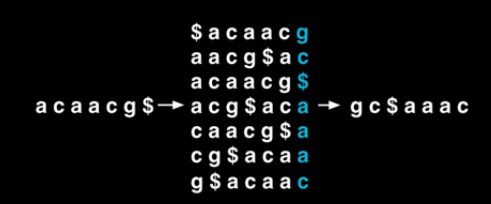
\includegraphics[width=0.6\textwidth]{1LF.png}
\caption{}
\end{figure}

\begin{figure}[h]
\centering
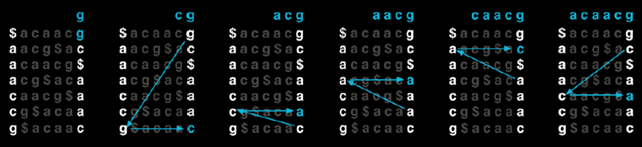
\includegraphics[width=0.6\textwidth]{2LF.png}
\caption{}
\end{figure}

\begin{itemize}
    \item \emph{g} is the first occurrence of g in the last column and corresponds to (arrow) the first occurrence of \emph{g} in the first column. Tracing a horizontal arrow gives the next nucleotide.
    \item \emph{c} is the second occurrence in the second column and corresponds to (arrow) the second occurrence of \emph{c} in the first column. Tracing an horizontal arrow gives the next nucleotide.
    \item \emph{a} is the third occurrence of a in the second column and corresponds (arrow) to the third occurrence of \emph{a} in the first column. Tracing an horizontal arrow gives the next nucleotide.
\end{itemize}

And so on. Each time we keep track of the character that we are looking at and we end up by constructing the original word. With this method we reconstruct the word from its end to its beginning (backward). 

\subsection{Exact mapping using LF property}

In mapping, we can look for sequence matches using the compressed database.
Backward exact mapping works by calculating the range of matrix rows beginning with successively longer suffixes of the query.
Example: we want to match the string 'aac' with the database.

\begin{figure}[h]
\centering
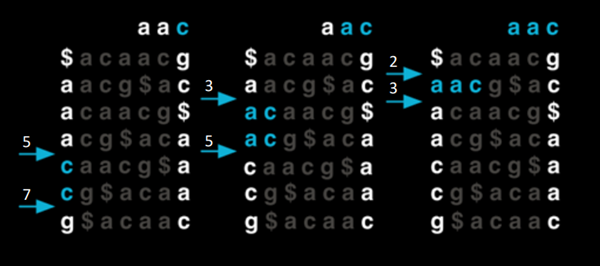
\includegraphics[width=0.6\textwidth]{3LF.png}
\caption{}
\end{figure}

\begin{itemize}
    \item we take the 'first suffix' \textbf{c} of the query string and we look for it in the first column. We find 2 matches in lines 5 and 6, so in the range 5-7.
    \item we pass to a 'second longer suffix' \textbf{ac} and see if we can find it in the matrix $\xrightarrow[]{}$ lines 3 and 4, range 3-5.
    \item we look at the suffix \textbf{aac} and find it in the 2-3 range.
\end{itemize}

Doing the backward matching we exploit the characteristics of the BWT transform. This same approach could be used to find a match between a query read and a reference genome which has been compressed using the BW alignment.
The problem is that it does not take into accounts indels, mismatches. 
A possible solution to this problem could be the \textbf{inexact mapping}. 
Perform exact mapping and, if the query is not found, go back and perform backtracking by hypothesising mismatches. For example we want to find a match for the query GGTA. As always, we start looking for a match starting from the last character.

\begin{itemize}
    \item we find a match for a, t, g but not for the last g. 
    \item so we go back and hypothesize a mismatch for the first letter a. We then look for all the matches that we could find if we replace a with another nucleotide (we do the same for the other NTs in the query?). 
    \item we find than by replacing a with a g, we find a match (ggtg) (not exact match).
\end{itemize}

The Burrows-Wheeler algorithm is used in BowTie and Bowtie2. 
Right now there are many algorithms to choose between and many review papers compare their characteristics and performance. No tool outperforms the others in all the test, hence the decision of which algorithm to choose must depends on the specific needs. 

\begin{figure}[h]
\centering
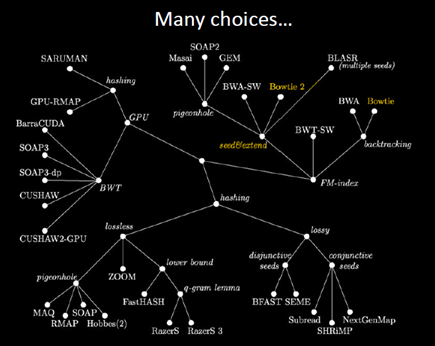
\includegraphics[width=0.6\textwidth]{Choices.png}
\caption{}
\end{figure}

\chapter{Assembly}

\graphicspath{{chapters/images/07/}}
\chapter{16S-rRNA sequencing}

\section{Introduction to metagenomics}

  \subsection{Definition of metagenomics}
   The term metagenomics refers to the study of uncultured microorganisms from the environment, which can include humans or other living hosts with focus on taxonomic and functional characteristics of the total collection of microorganisms within a community.
   The main way to analyse the entire microbial population of an environment is through high-throughput sequencing of nucleic acids isolated from the sample.
   Two approaches can be distinguished:

   \begin{multicols}{2}
     \begin{itemize}
       \item 16S rRNA gene sequencing.
         \item Shotgun metagenomic.
     \end{itemize}
   \end{multicols}

  \subsection{Why studying the metagenome}
   Microbes are basically everywhere, in and outside of our bodies, in oceans, glaciers, hot springs and rocks.
   Given how widespread and abundant microbes are, studying the metagenome provides us plenty of information both on human and non-human microbiome and environment.
   For instance, it has been shown that the microbiome correlates to several diseases, therefore it can be used as a non-invasive biomarker.
   The list of activities microbes are involved in is constantly increasing.

  \subsection{Differences with older microbiome studies}
  The microbiome was discovered many years ago but there were no tools to analyze it properly: the only way was to culture and isolate each bacterium.
  This is an unfeasible approach to study the entire community, since only some bacteria can be grown in the laboratory and it would take an unreasonably long amount of time.
  The advent of high-throughput technologies is what made possible to study the microbiome of a sample, reducing significantly times, costs and increasing substantially the fraction of the microbiome that can be known.

  \subsection{Example: skin microbiome}
  Some studies were performed on skin microbiome (Segata et al, Nature Methods 2012, Truong et al, Nature Methods, 2015).
  Only about $60\%$ of the contigs of various size were mapped to known microbes while $40\%$ belonged to unknown species.
  When separating these sequences based on GC content and abundance, many clusters formed, some with higher abundance while others with lower abundance, probably due to the low GC content that makes more difficult for the machine to sequence them, therefore causing them to be underestimated.
  Studying this $40\%$ of unknown sequences is one of the main tasks of metagenomics.

\section{16S rRNA sequencing}
16S rRNA sequencing is one of the first techniques developed to study the microbiome, since it does not require a huge amount of sequences nor excessive costs.

  \subsection{Simplified 16S rRNA analysis workflow}
    The general workflow for a 16S rRNA analysis is the following:

    \begin{multicols}{2}
      \begin{itemize}
        \item DNA extraction from the entire community present in the sample.
          Some bacteria will be over-represented while other will be under-represented.
        \item Selective PCR amplification of 16S rRNA gene.
        \item High-throughput sequencing.
        \item Sequence mapping against genomes in databases.
          This allows to define which bacteria and which variants of those are present in the sample and to find new and unknown bacteria.
      \end{itemize}
    \end{multicols}

    \begin{figure}[H]
      \centering
      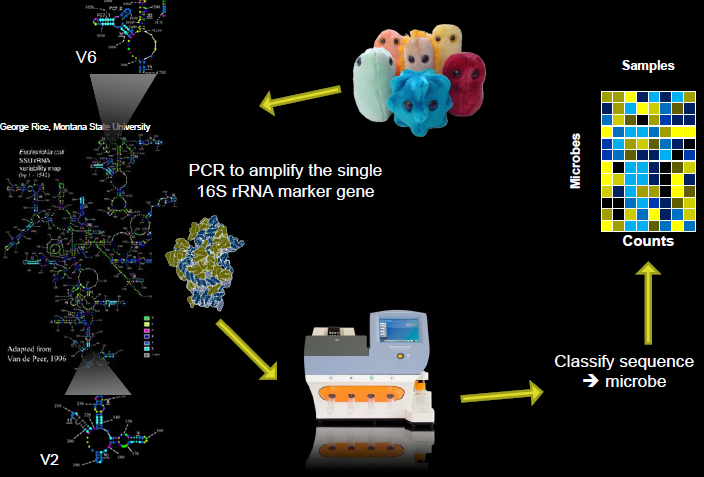
\includegraphics[width=0.9\textwidth]{general_workflow.png}
      \caption{\label{fig:general_workflow}General 16S gene analysis workflow}
    \end{figure}

  \subsection{16S rRNA gene}
    The ribosome is one of the most conserved, if not the most conserved, structure in all living organisms, making it one of the best phylogenetic markers.
    In prokaryotes, the ribosome is composed of several elements, both proteic and RNA based.
    Of the RNA based ones, $3$ of them are ribosomial RNAs (rRNAs), namely 5S, 16S, 23S.
    Since these components are fundamental for any bacterium, all bacteria present the genes codifying for these rRNAs.
    Moreover most of the sequences are highly conserved but some regions have some species-specific variability which can be used as a barcode to find and classify species.
    The most conserved of the rRNAs is 23S but the one used for microbiome analysis is 16S (which corresponds to the human 18S).
    Its gene is a few thousands nucleotides long, most of which are highly conserved.
    The bulk of the differences among species is in the hypervariable regions named V1 to V9, the terminal loops of the structure.
    They are regions far away from the catalityc site.
    Despite the high degree of conservation, some variability can be found outside the hypervariable regions too.
    The annotation of which portions of the 16S rRNA gene are conserved has been performed using E. coli as a reference.
    For a few hundred organisms the gene has been compared to the reference one to define the degree of conservation of each stretch of nucleotides.
    Some totally conserved regions  are present but they are not very big.

    \begin{figure}[H]
      \centering
      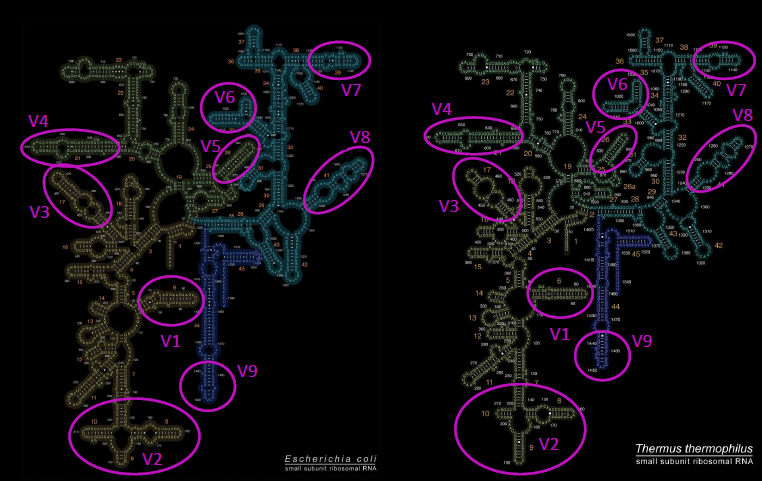
\includegraphics[width=0.9\textwidth]{16S_rRNA.png}
      \caption{\label{fig:16S_rRNA}Structure of the 16S rRNA in \textit{E. coli} and \textit{T. termophilus}}
    \end{figure}

  \subsection{Primer and high-throughput machine choice}
    One could sequence the entirety of the 16S rRNA gene, for example using NanoPore seq, but this would introduce many errors that could lead to mapping the sequence to the wrong organism.
    For this reason it is preferred to amplify only certain specific regions of the gene.
    To study the microbiome in a high-throughput way primers which can bind to all species are needed.
    Since the sequences conserved in all species are too short, you use primers that bind highly conserved regions.
    For this reason, regardless of which primers you choose there will be a bias in your results: some species will not be identifiable using those primers.
    This bias can be somewhat minimized using in silico primer validation, which means testing your primers against databases of 16S tRNA genes like silva and green genes, to test and decide the best pair of primers for your experiment.

    \begin{figure}[!h]
      \centering
      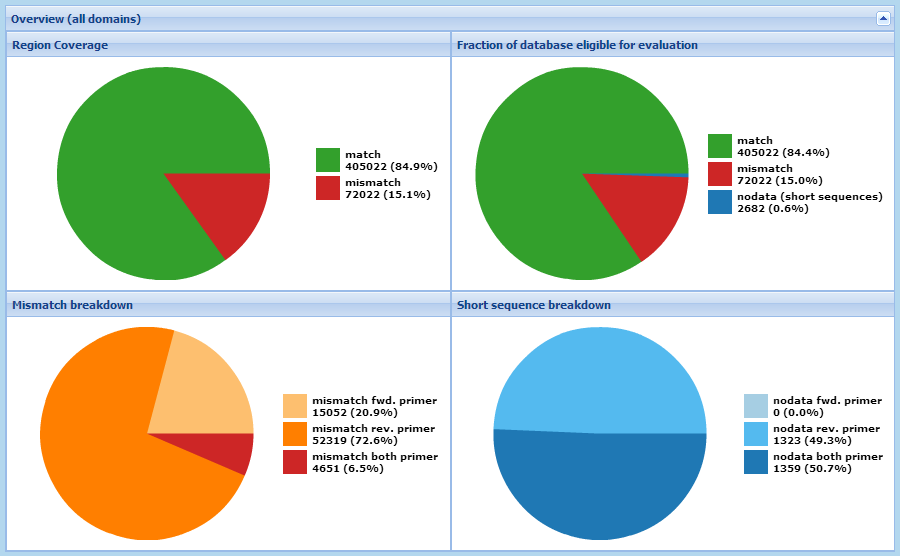
\includegraphics[width=0.9\textwidth]{silva_analysis.png}
      \caption{\label{fig:silva_analysis}Example of \textit{in silico} primer validation using silva; you can notice the different efficiency of the primers relative to different parameters.}
    \end{figure}

    Still, two experiments conducted with different primers will always have some differences.
    Moreover the binding regions must flank some variable region, in order to include it in the amplicon.
    Finally pair end amplification both primer back and forward is needed in order to have the complete amplicon to make the comparison easier.
    Given these characteristics there are multiple possible priming sites based on the sequence and on chemical properties of the primers.
    Moreover, primers can be used as forward or reverse to obtain different combinations and sequences.

    \begin{figure}[!h]
      \centering
      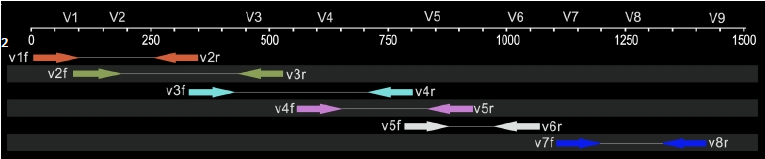
\includegraphics[width=0.9\textwidth]{primer_placement.png}
      \caption{\label{fig:primer_placement}Examples of common primer placements relative to hypervariable regions}
    \end{figure}

    As an example of the importance of the choice of primers, in some skin microbiome analyses, researchers could not find two bacteria always present on human skin due to the choice of primers.
    Moreover S. aureus seemed over-represented due to the non-amplification of other important species.
    Despite the biases, this technique is still extremely useful.

    There are different protocols to target conserved regions also based on the machine used.
    In general:

    \begin{multicols}{2}
      \begin{itemize}
        \item Sanger machines are not very good for this application since they have low throughput and they are more suited for longer sequencing tasks.
        \item Roche 454 machines have historically been well suited, since it was possible to sequence three hypervariable regions together using $400$ nucleotides reads, providing a good cost and throughput trade-off.
        \item Illumina HiSeq is not the optimal choice since it has shorter reads and unnecessarily high throughput.
          Illumina MiSeq and IonTorrent can be a decent compromise.
      \end{itemize}
    \end{multicols}

  \subsection{In depth 16S rRNA analysis workflow}
  Adding detail, a more complete overview of the 16S rRNA analysis workflow is:

  \begin{multicols}{2}
    \begin{itemize}
      \item DNA extraction from each of your samples
      \item Selective PCR amplification of 16S rRNA gene, introducing a barcode in the sequences using tagged primers.
      \item High-throughput sequencing of all the samples in a single run to reduce costs.
        The result is a set of amplicons belonging to different samples and with a barcode attached.
      \item Demultiplexing, which means removing the barcodes and assigning each sequence  to the corresponding sample.
        Sequencing noise must be taken into account, therefore low quality reads must be removed.
      \item Multiple sequence alignment against reference sequences.
        Some reads will probably not map to any reference sequence.
      \item Group related sequences into OTUs (operational taxonomic units), which means grouping sequences that share some common variants.
        Since SNPs in the microbial genome are present, the similarity threshold between sequences cannot be too restrictive.
        OTUs can be used to define the relative abundance of each species in the sample, but in order to do so it is necessary to normalize for the copy number of the 16S gene sequence.
        This is very difficult since an accurate estimate can be made only if long read sequencing has been performed on the organism, which is almost never the case since for microbes that basically corresponds to full genome mapping.
      \item Build phylogenetic tree using one representative for each OTU.
      \item Annotate the OTUs using 16S gene databases.
      \item Downstream analysis is performed, such as clustering to visualize similarities among samples.
    \end{itemize}
  \end{multicols}

    \begin{figure}[!h]
      \centering
      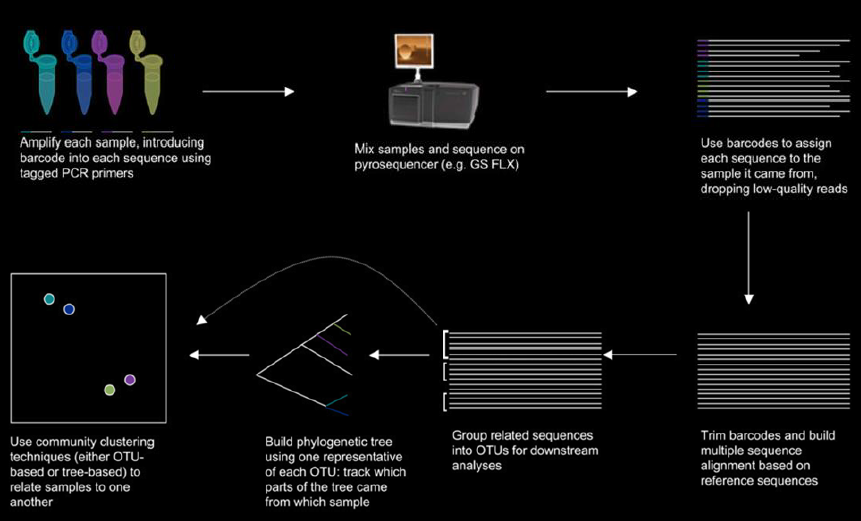
\includegraphics[width=0.9\textwidth]{expanded_workflow.png}
      \caption{\label{fig:expanded_workflow}Expanded 16S gene analysis workflow}
    \end{figure}

    \begin{figure}[!h]
      \centering
      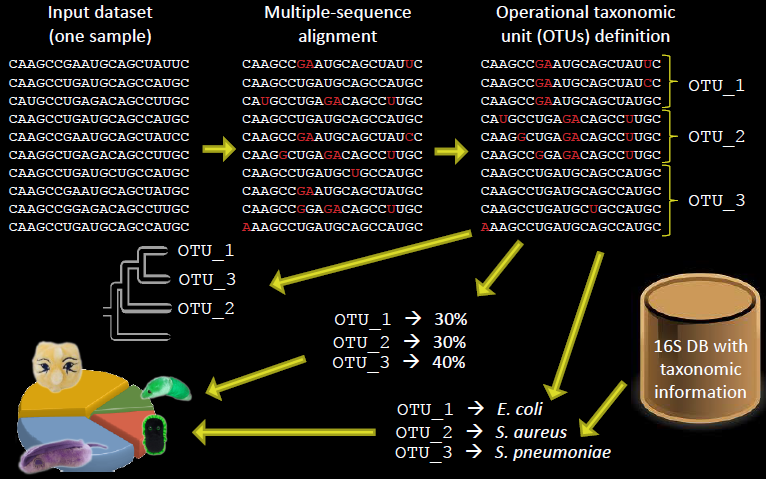
\includegraphics[width=0.9\textwidth]{zoom_in_16S.png}
      \caption{\label{fig:zoom_in_16S}Zoom in on 16S gene analysis workflow}
    \end{figure}

  \subsection{OTU clustering}
  Defining OTUs requires using multiple sequence alignment.
  Since this approach is a generalization of the mapping algorithm it is quite complex in terms of speed, but still feasible.
  Generally greedy algorithms which add the lowest possible amount of gaps are used to perform multiple sequence alignment.
  After the alignment, sequences are split into OTUs (operational taxonomic units), which are groups of 16S sequences very similar to each other.
  Generally a sequence is defined as the representative of the OTU, meaning that it has a certain threshold of identity with all other sequences in the OTU, usually $97\%$ when considering species and that minimizes the differences of all other sequences of the OTU with itself.
  Some OTUs can be assigned univocally to a species, some others may be associated to more species, some others cannot be mapped to know species.
  The fact that a species may map to multiple OTUs is often an error but it may sometimes allow to find subspecies.

    \begin{figure}[!h]
      \centering
      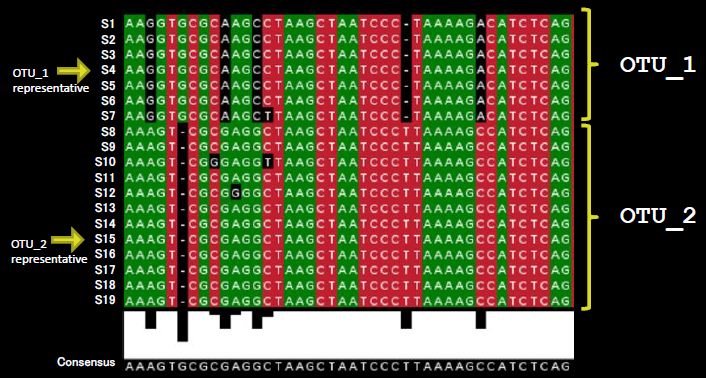
\includegraphics[width=0.9\textwidth]{OTU_general.png}
      \caption{\label{fig:OTU_general}Example of multiple sequence alignment for OTUs}
    \end{figure}

    After sequence alignment, OTU clustering can be done through several supervised or unsupervised learning methods.
    The most common unsupervised clustering methods are:

    \begin{multicols}{2}
      \begin{itemize}
        \item Single linkage clustering nearest neighbour: assign the sequence to a cluster if that OTU already contains at least a sequence similar enough ($97\%$).
          However two distant sequences in the OTU network could share a similarity which is way lower than $97\%$.
          This could result in underclustering.
        \item Complete linkage clustering furthest neighbour: assign the sequence to a cluster only if all the sequences of the OTU are similar enough ($97\%$).
          However two sequences may be similar enough, yet belong to different OTUs, because the overall cluster width, or divergence, is at most $3\%$.
          This approach could then generate different solutions, based on the order the points are added in.
          Moreover, if the clustering conditions are too stringent, sequencing errors and SNPs in the microbial genome may result in overclustering (defining too many clusters).
      \end{itemize}
    \end{multicols}

    \begin{figure}[!h]
      \centering
      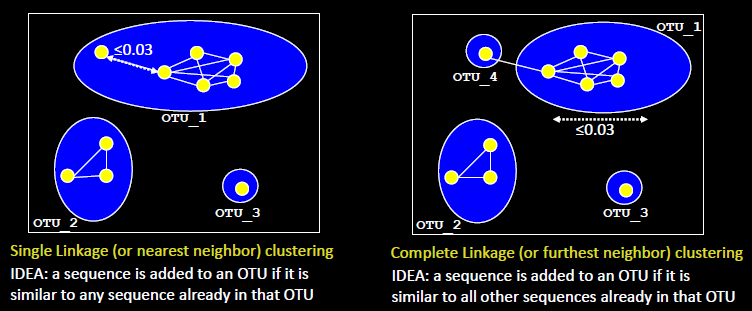
\includegraphics[width=0.9\textwidth]{clustering_methods.png}
      \caption{\label{fig:clustering_methods}Visualization of single linkage analysis and complete linkage analysis}
    \end{figure}

    \begin{figure}[!h]
      \centering
      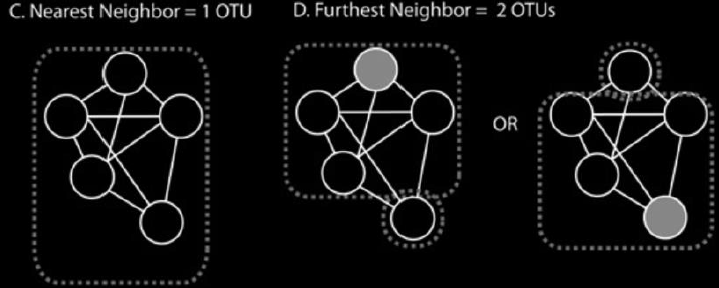
\includegraphics[width=0.9\textwidth]{overclustering.png}
      \caption{\label{fig:overclustering}Example of overclustering and result multiplicity due to complete linkage analysis}
    \end{figure}

  \subsection{OTU taxonomic annotation}
  Assigning a taxonomic annotation to an OTU cannot be done simply using BLAST to get the best matching sequence.
  This is because there is too much noise in the sequences and because it is difficult to classify new strains.
  A better way is using some other algorithm that assigns the terms of the taxonomic notation (since it is more than just one label) and provides some degree of confidence in the prediction.
  For instance the algorithm may be able to correctly assign the first taxonomical terms, up until Enterobacteriaceae, but then it provides a prediction of the OTU belonging to a list of species with confidence value for each one.

    \subsubsection{RDP classifier (Naive Bayes Model)}
    $P(S|G)$ is computed by RDP using a 8-mer strategy: comparing the 8-mers in $S$ with the 8-mers in all the training sequences available for genus $G$.
    The confidence of each prediction is computed by bootstrapping:

    \begin{multicols}{2}
      \begin{enumerate}
          \item Select a random subsequence of $S$, $S’$.
          \item Compute the $G$ that maximizes $P(S’|G)$.
          \item Repeat the procedure a number of times.
          \item The number of time $G$ is selected by the bootstrapping procedure is the confidence
      \end{enumerate}
    \end{multicols}

    Leave one-out-cross validation:

    \begin{multicols}{2}
      \begin{itemize}
          \item Take out one data point from the training set.
          \item Apply the classifier on the left-out point (without using it in the training set).
          \item Check the accuracy of the prediction.
          \item Repeat the procedure for each training data point.
      \end{itemize}
    \end{multicols}

    The RDP classification accuracy is evaluated with the leave-one-out cross validation on the training set of hundreds thousands of 16S references:

    \begin{multicols}{2}
      \begin{itemize}
          \item Accuracy is the percentage of correct classification (over the all leave-one-out runs).
          \item There are varying levels of taxonomic resolution (from phylum to genus).
          \item There are varying sequence lengths.
          \item In real applications accuracies are probably smaller due to sequencing errors or the presence of unknown bacteria.
      \end{itemize}
    \end{multicols}

\section{Diversity analysis}

\begin{figure}[h]
  \centering
  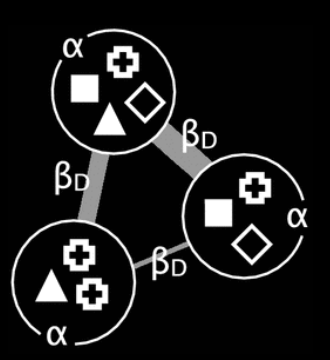
\includegraphics[width=0.6\textwidth]{Diversity.png}
  \caption{}
\end{figure}

  \subsection{Alpha diversity analysis}
  Alpha diversity analysis is a measure of how diverse or complex a microbial community is.
  It measures within sample diversity.
  Species richness is a widely use alpha diversity index.
  All individuals considered have non-zero abundance, some will have high abundance ($\sim99\%$) or low abundance ($1\%$).
  High alpha diversity are usually associated with populations that are more robust and resilient to changes.
  For examples gut microbiome with a high richness is usually associated with healthy state, instead of disease.
  Alpha diversity can be compared only between samples with the same sequencing depth.
  To do so between different samples usually a depth cut-off is chosen.

  \subsection{Beta diversity analysis}
  Beta diversity analysis is a measure of how different two microbial communities are.
  It measures between sample diversity.
  It is possible to measure the beta-diversity using the inverse of number of shared species.
  An example of beta-diversity is UniFrac.
  In UniFrac the distance is equal to the fraction of the total branch length that is unique to any particular environment.
  UniFrac can be also weighted in order to include abundances for each OTU.

  \begin{figure}[h]
    \centering
    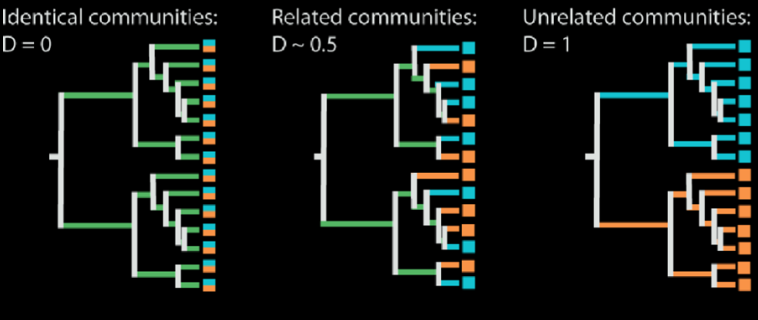
\includegraphics[width=0.6\textwidth]{UniFrac.png}
    \caption{\textbf{D=0.} Blue and orange samples always have the same OTUs. Each 16S (each branch) is present in both samples. \textbf{D=$\sim$0.5.}In reality we usually have a mix of the 2 situations. Some OTUs are present only in one of the samples and are either quite distant from the others or close (based on upstream the branch goes). \textbf{D=1.} Completely distinct OTUs . The difference is also in the upstream branches, which have different colors.}
  \end{figure}

  \subsection{Principal Coordinate Analysis}
  PCoA is also known as multidimensional scaling.
  It is one of the most powerful approaches for exploratory analysis.
  The idea is to represent the multidimensional relationship between samples in a two or three dimensional space.
  It is possible to use any similarity function as Euclidean distance, UniFrac, bray-Curtis distance.
  We find frequently hierarchical clustering plots.
  It is mostly done to visualize the similarities and difference between species, identifying for example cluster of species.

\graphicspath{{chapters/images/08/}}

\chapter{Shotgun Metagenomics}

\section{Introduction}

    \subsection{Shotgun metagenomic analysis}
    A shotgun metagenomic analysis consists of different steps:

    \begin{multicols}{2}
        \begin{itemize}
            \item Experimental pipeline: from sample collection to DNA sequencing.
            \item Preprocessing:  decontamination and quality control.
            \item Mapping, assembling or both.
            \item Sequence analysis:  identification of microbial species and identification of present pathways and functions.
            \item Post Processing: integrate data with other information coming from sample metadata.
            \item Validation:  follow-up experiments with independent replicates.
        \end{itemize}
    \end{multicols}

    \begin{figure}[!h]
        \centering
        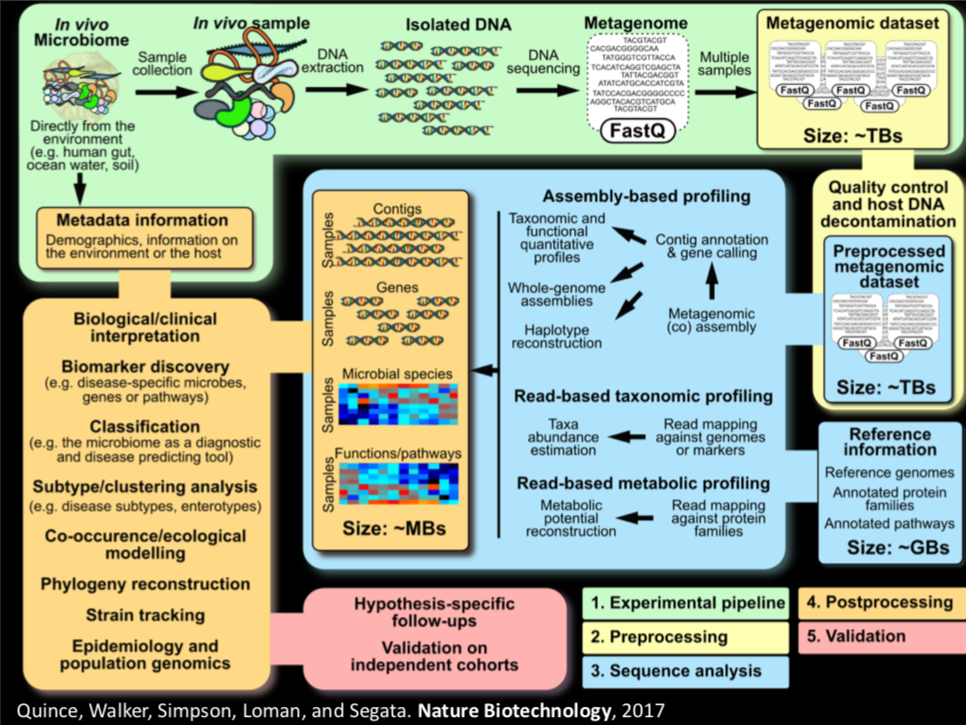
\includegraphics[width=0.9\textwidth]{Shotgun_workflow.png}
        \caption{\label{fig:workflow}Shotgun metagenomics workflow}
    \end{figure}

    \subsection{Comparison with the 16s sequencing}

    \begin{tabular}{ | m{7cm}| m{7cm} | }
     \hline
     \multicolumn{2}{|c|}{16S sequencing} \\
     \hline
     Pros & Cons \\
     \hline
     Cost-effective & Non genome-wide \\
     Avoids non-bacterial contamination & Limited taxonomic resolution \\
     Can catch low-abundance bacteria & Not useful for pathogens profiling \\
     The output has reasonable size and complexity & Does not detect viruses or eukaryotes \\
     Mature software available to perform the computations & Several biases\\
     & Cross studies are difficult: the comparison is not possible due to biases \\
     \hline\hline
     \multicolumn{2}{|c|}{Shotgun sequencing} \\
     \hline
     Pros & Cons \\
     \hline
     Genome-wide: it is possible to retrieve information about all the genes present in the metagenome & Expensive (but costs are decreasing: right now the cost for the sequencing of one sample is $\sim100\$$) \\
     High taxonomic resolution & DNA contamination are hard to remove \\
     Easy cross-study comparison thanks to the lack of biases & Low-abundance bacteria could be missed \\
     All domains of life can potentially be observed in the same study & Large dataset as output, that can be difficult to process (TBs of data) \\
     \hline
    \end{tabular}

    \subsection{Latest technology}
    The cost of $100\$$ for the sequencing of one sample refers to a sample size of $5Gb$, that should be enough for shotgun metagenomics.
    More sequencing depth could be needed if microbes with very low abundances needs to be detected, if many new genomes need to be assembled or if there is a lot of contamination.
    Shotgun metagenomics is possible with Illumina Hiseq technology, but the latest and most used technology nowadays is Illumina NovaSeq.

\section{Identification of microbes from Shotgun metagenomics data}
The main challenges with respect to identifying microbes from metagenomics data are:

\begin{multicols}{2}
    \begin{itemize}
        \item How to obtain species-specific resolution.
        \item Computational feasibility.
        \item Being able to detect both bacteria and archaea.
            Phages are also a problem since there is little reference.
        \item Obtain relative abundances of organisms with different genome sizes.
        \item Consistent detection confidence for all clades.
        \item How to handle reads as short as $50nts$.
        \item Detect organisms without a sequenced genome or still unknown species.
    \end{itemize}
\end{multicols}

    \subsection{MetaPhlAn: unique marker genes for taxonomic profiling}
    The main idea of MetaPhlAn is to find a marker gene that uniquely characterizes a species.
    This gene has to be present in all strains of a species and in no other species.
    This markers form taxonomic clades.
    ChocoPhlAn is the tool that generates the database necessary.
    From a number of genomes, ChocoPhlAn was used to create a database of marker genes that build the MetaPhlAn database.
    This database contains $200$ markers per species and its reduced dimension with respect to the whole genomes database can align reads directly to the marker database.

    \begin{figure}[!h]
        \centering
        \includegraphics[width=0.95\textwidth]{MetaPhlAn.png}
        \caption{\label{fig:metaphlan}MetaPhlAn overview}
    \end{figure}


        \subsubsection{Creation of the marker genes database}
        The marker database was created from $2887$ genomes from $1222$ species.
        The number of marker per species decreases with more sequenced genomes because the core genome tends to become smaller in size and noise is eliminated.
        In the current version $1$ milion genomes are considered, with $200000$ isolated genomes and $800000$ from metagenomics assembled genomes or MAGs.

        \subsubsection{Efficiency and validation}
        MetaPhlAn can deal with $200000$ reads per second and can profile thousands of microbiomes in a few hours.
        Validation can be done with synthetic metagenomes created with errors or with biological methods: comparing the results with the ones obtained with 16S based abundance estimations.

        \subsubsection{The problem of the unknowns}
        Microbial species that were never observed and do not have a marker in the database cannot be detected with this method.
        A possible solution is to cluster together contigs obtained from the metagenome based on coverage, GC content, codon bias, and other possible features.
        Strict quality controls are then performed on these putative genomes: on the number of genes and the number of known single-copy genes in order to be sure that what has been found is not a mixture of genomes.
        High quality putative genomes are considered MAGs and version 4 of MetaPhlAn can include them in the creation of the marker database.
        This way, these species can be detected in metagenomes even though they do not have a name yet.

    \subsection{Other approaches}
    Other approaches include:

    \begin{multicols}{2}
        \begin{itemize}
            \item Sequence-based clustering of contigs to create putative genomes.
                The output are unlabelled bins with relative abundances.
                The main problem is that high coverage is needed to obtain valid results.
            \item Machine learning algorithms that exploit GC content (and possibly other features) to give as output clades with relative abundances.
                This method is not completely reference-free as it uses reference genomes to extract the features used for the classification.
                The main problem is that many species could have really similar features.
            \item Read-to-genome sequence mapping.
                In this approach there is no processing of a reference genome.
        \end{itemize}
    \end{multicols}

    \begin{figure}[H]
        \centering
        \includegraphics[scale=0.3]{taxApproaches.png}
        \caption{\label{fig:taxApproaches}An overview of taxonomic profiling approaches}
    \end{figure}

    \subsection{The curated MetagenomicData resource}
    Since raw metagenomic sequencing data can be quite difficult to deal with computationally, the curated metagenomic data database stores features obtained from raw metagenomic datasets uniformly processed (MetaPhlAn or HUMAnN2) and integrated with associated metadata obtained from NCBI, papers and authors.
    This database is accessible and can be exploited to perform various types of analysis.

    \begin{figure}[!h]
    \centering
    \includegraphics[width=0.4\textwidth]{curatedMetagenomicData.png}
    \caption{\label{fig:curatedMetagenomicData}CuratedMetagenomicData pipeline}
    \end{figure}

    \subsection{The link between the gut microbiome and colorectal cancer}
    Colibactin is a genotoxic metabolite produced by E. coli: it causes damages to the DNA, possibly causing cancer onset.
    A fraction of human colorectal cancer (CRC) cases are caused by colibactin.
    A study published by Segata’s group collected stool samples from people having a colonoscopy in Milan (\ref{fig:milanCRC}) and Turin (\ref{fig:turinCRC}).
    The samples were then categorized after the diagnosis provided by the colonoscopy.
    The aim was the identification of biomarkers associated with the CRC phenotype.
    Different results were obtained in the two cities.

    \begin{figure}[!h]
    \centering
    \begin{subfigure}{.45\textwidth}
        \centering
        \includegraphics[width=\linewidth]{MilanCRC.png}
        \caption{\label{fig:milanCRC}Patients from Milan}
    \end{subfigure}
    \begin{subfigure}{.45\textwidth}
        \centering
        \includegraphics[width=\linewidth]{TurinCRC.png}
        \caption{\label{fig:turinCRC}Patients from Turin}
    \end{subfigure}
    \caption{Taxonomic profiling of gut microbiomes}
    \end{figure}

    Comparing this study with similar ones performed around the world (France, China, Austria, USA, Germany and Japan) some biomarkers appeared to be reproducible (\ref{fig:biomarkers}).
    Moreover, an accuracy around $80\%$ was observed when a machine learning approach (random forest) was applied on all the datasets combined and then the model was applied on a brand new one(\ref{fig:ML}).
    On the other hand, when each group tried the same approach on their data separately, completely different results were found for each dataset, showing that such a technique could be valid for some cases and completely unhelpful for others.

    \begin{figure}[!h]
    \centering
    \begin{subfigure}{.45\textwidth}
        \centering
        \includegraphics[width=\linewidth]{CRCbiomarkers.png}
        \caption{\label{fig:biomarkers} \emph{F. nucleatum} found to be enriched in datasets with different origins}
    \end{subfigure}
    %
    \begin{subfigure}{.45\textwidth}
        \centering
        \includegraphics[width=\linewidth]{CRC_ML.png}
        \caption{\label{fig:ML}Random forest approach on all the datasets shows an accuracy of $0.80$ (AUC of $1$ means always right prediction, $0.5$ means no prediction ability)}
    \end{subfigure}
    \caption{}
    \end{figure}


        \subsubsection{Hypothesis-driven analysis}
        The cutC gene appears to be associated with the CRC phenotype (\ref{fig:cutC}).
        The problem is that it is present in several microbial species and it is unknown whether the function and the efficiency are maintained.

        \begin{figure}[H]
            \centering
            \includegraphics[scale=0.2]{cutC.png}
            \caption{\label{fig:cutC}}
        \end{figure}

    \subsection{PanPhlAn: strain-level profiling}
    PanPhlAn is a tool for strain-level metagenomic profiling that allows to identificate gene composition of individual strains in metagenomic samples.
    The main difficulties to consider with this approach are:

    \begin{multicols}{2}
        \begin{itemize}
            \item Identify the microbial strains present in the metagenome or check whether a specific one is present in the sample.
            \item Discover new strains and species.
            \item Characterize the metagenome genomically.
            \item Track across samples to find the same strain and eventually prove that transmission of bacterial strains occurred among them.
        \end{itemize}
    \end{multicols}

    Let's consider an analysis regarding the \emph{E. coli} pan genome contains about 20.000 gene-families.
    The goal is to find what strains are present in the metagenome and their abundances.
    First all genes are grouped in functional gene-families (\ref{fig:pan1}).
    Then genes from \emph{E. coli} found in the metagenome are mapped on \emph{E. coli} reference genomes with BowTie2.
    The coverage is computed for each gene and then they are grouped into gene-families (\ref{fig:pan2}).
    Then gene-families are ranked based on their coverage.
    Multi-copy gene families have really high coverage, while the plot shows a plateau of single-copy gene-families.
    These families correspond to the strains present in the metagenome and their abundance can be deducted thanks to the base coverage of single-copy genes.

    \begin{figure}[!h]
    \centering
    \includegraphics[width=0.9\textwidth]{panphlan1.png}
    \caption{\label{fig:pan1}Genes are grouped in functional gene-families}
    \end{figure}

    \begin{figure}[!h]
    \centering
    \includegraphics[width=0.9\textwidth]{panphlan2.png}
    \caption{\label{fig:pan2}Mapping and subsequent coverage of gene-families}
    \end{figure}

    \begin{figure}[!h]
    \centering
    \includegraphics[width=0.6\textwidth]{Coverage.png}
    \caption{\label{fig:pan3}\emph{E. coli} gene-family distribution: curve (A) shows the typical gene-families distribution: multi-copy genes with extremely high coverage, a plateau of single-copy genes and a tail of non-present gene-families. Curves like (C ) should be discarded from the analysis because they indicate that no \emph{E. coli} strain is detected in that sample.}
    \end{figure}

        \subsubsection{Investigating population genomics thanks to PanPhlAn}

            \paragraph{\emph{E. coli} population genomics with PanPhlAn}
            Figure \ref{fig:Ecoli1} shows the \emph{E. coli} profiling of 1478 shotgun metagenomes carried out with PanPhlAn.
            Each column is either an \emph{E. coli} strain obtained via shotgun metagenomics or a reference strain and the columns correspond to the gene-families that can be absent or present in each strain.
            The strains are then clustered (\ref{fig:Ecoli2}) based on which gene-families are present in order to study the population genomics: in this case we can see that the strains isolated from the German \emph{E. coli} outbreak cluster together, while other strains are present in several different areas of the world.

            \begin{figure}[!h]
            \centering
            \begin{subfigure}{.49\textwidth}
                \centering
                \includegraphics[width=\linewidth]{Ecoli1.png}
                \caption{\label{fig:Ecoli1}}
            \end{subfigure}
            %
            \begin{subfigure}{.49\textwidth}
                \centering
                \includegraphics[width=\linewidth]{Ecoli2.png}
                \caption{\label{fig:Ecoli2}}
            \end{subfigure}
            \caption{\emph{E.coli} population genomics with PanPhlAn}
            \end{figure}

            \vspace{2cm}

            \paragraph{PanPhlAn on \emph{Eubacterium rectale}}
            Thanks to PanPhlAn, it was possible to identify many subtypes of \emph{E.rectale} even though only one reference genome was available at the time (\ref{fig:Erec}).

            \begin{figure}[!h]
            \centering
            \includegraphics[width=0.6\textwidth]{Erectale.png}
            \caption{\label{fig:Erec} PanPhlAn on \emph{Eubacterium rectale}}
            \end{figure}

            \paragraph{The infant gut microbiome in disease}
            Necrotizing Enterocolitis (NEC) is a devastating disease that affects mostly the intestines of premature infants.
            This study took samples from a cohort of 173 infants, 151 of them were preterm and 30 of them had NEC.
            They obtained 460 shotgun metagenomic samples and 284 shotgun metatranscriptomic samples, all of which were coupled with clinical data of the patients.
            The heatmap shows MetaPhlAn profiling of different bacterial species for all the samples: about 20\% of the patients have a high \emph{E. coli} predominance (\ref{fig:nec1}: yellow circle).
            PanPhlAn was employed to investigate the \emph{E. coli} strains found in these patients: of the 4 identified clades, only 2 are associated with NEC (\ref{fig:nec2}).

            \begin{figure}[!h]
            \centering
            \begin{subfigure}{.45\textwidth}
                \centering
                \includegraphics[width=\linewidth]{nec1.png}
                \caption{\label{fig:nec1}MetaPhlAn2 profiling of the cohort of infants}
            \end{subfigure}
            %
            \begin{subfigure}{.45\textwidth}
                \centering
                \includegraphics[width=\linewidth]{nec2.png}
                \caption{\label{fig:nec2}PanPhlAn to resolve NEC-assocated E. coli diversity}
            \end{subfigure}
            \caption{The infant gut microbiome in disease}
            \end{figure}

    \subsection{StrainPhlAn}
    The idea in which StrainPhlAn is based on is to base the classification on the genetic variance of core genomes: look for unique combinations of SNPs in genes that are always present and analyse their variance to find some SNPs with a variance different from the others that could characterize a new strain.
    StrainPhlAn exploits MetaPhlAn to compute species-level abundances thanks to species-specific markers and then aligns the marker genes present in the samples to find the SNPs.
    The SNPs are then analysed to build a phylogenetic tree.
    This approach can be applied to many different species.
    For example studies concerning \emph{E. rectale} seems to have a higher resolution compared to the previous approach.

    \begin{figure}[!h]
    \centering
    \includegraphics[width=0.9\textwidth]{StrainPhlAn.png}
    \caption{\label{fig:strainphlan}StrainPhlAn pipeline}
    \end{figure}

        \subsubsection{StrainPhlAn applications}

            \paragraph{The stability of strains in the human gut}

            \begin{figure}[!h]
            \centering
            \includegraphics[width=0.8\textwidth]{strainGut.png}
            \caption{\label{fig:gut}The stability of strains in the human gut}
            \end{figure}

            This study analyses samples of the human gut microbiome obtained from different continents.
            The barplots (\ref{fig:gut}) show the distances measured between results of SNPs analysis in different regions around the world.
            There are almost no pairs with zero or low distance and the results do not change if only subjects from the EU or US are considered.
            On the other hand, the red and blue barplots (\ref{fig:gut}) show that comparing the SNPs of samples coming from the same individual but collected 6 months apart they show great similarity.
            This indicates that there is some stability in the human gut microbiome: usually the strains present in one’s gut microbiome tend to remain almost the same.
            Nevertheless, changes of diet or other habits can bring variations in their abundances.

            \paragraph{Identification of subspecies}

            \begin{figure}[!h]
            \centering
            \includegraphics[width=0.5\textwidth]{strainGeo.png}
            \caption{\label{fig:geo}Association of sub-species structures with geography}
            \end{figure}

            Some bacteria are strongly represented in the human population’s microbiomes and their presence is detected in all continents.
            On the other hand subspecies tend to be highly region-specific.
            In Figure \ref{fig:geo}, each color indicates a different country: it is clear that when looking at subspecies of these common microbes, they are mostly associated with only one country or continent.

    \subsection{Uncharacterised species}
    A great amount of information about the human is still unknown:

    \begin{multicols}{2}
        \begin{itemize}
            \item Functional unknowns: genes for which we still do not know the function because they do not match any functional database.
            \item Unknown species/strains: genes not matching any of the known reference genomes.
            \item Undetected unknowns: things we do not know and were not even observed yet.
        \end{itemize}
    \end{multicols}

    \subsection{Workflow for large scale metagenomic assembly}

    Westernized metagenomes are more characterized than non-westernized ones and this study performed a large scale metagenomic assembly on data from undercharacterized region of the world.
    They were able to reconstruct $\sim 70.000$ high quality genomes and $\sim 85.000$ medium-quality ones (with $~50\%$ completeness).

        \subsubsection{Project pipeline}
        Workflow (\ref{fig:workflow2}):

        \begin{multicols}{2}
            \begin{itemize}
                \item Assembly of the reads into contigs.
                \item Binning of contigs into putative genomes (MAGs = Metagenome-Assembled Genomes).
                \item Quality control.
                \item The MAGs are then clustered in species-level genome bins by measuring the distance scores between couples of putative genomes.
                \item SGB are divided into known, unknown and non-human.
            \end{itemize}
        \end{multicols}

        \begin{figure}[h]
        \centering
        \includegraphics[width=0.9\textwidth]{workflow2.jpg}
        \caption{\label{fig:workflow2}Workflow of large-scale metagenomic assembly}
        \end{figure}

        This study allow to characterize the new cibiobacter.
        In particular Madagascar associated strains of cibiobacter uniquely possess the trp operon for tryptophan metabolism.

\section{Applications of strain-level metagenomic profiling}

    \subsection{\emph{E.rectale} refined population genomics}

    \begin{figure}[!h]
    \centering
    \includegraphics[width=0.8\textwidth]{Erec2.png}
    \caption{\label{fig:Erec2}\emph{E.rectale} refined population genomics}
    \end{figure}

    Thanks to the advancements brought by strain-level metagenomic profiling, a new subtype of \emph{E. rectale} was discovered.
    Subtype 3 lacks the operon coding for motility and other genes that become useless for the bacteria if it is not motile.
    On the other hand, they present more copies of the CAZy genes: these are involved in metabolism and are required by non-motile bacteria in order to be more efficient in the exploitation of carbon sources since they cannot move to reach them.

    \subsection{\emph{Prevotella copri} is strongly lifestyle-associated}

        \begin{figure}[!h]
            \centering
            \includegraphics[width=0.8\textwidth]{Prevotella.png}
            \caption{\label{fig:prevotella}\emph{Prevotella copri} is strongly (Western) life-style associated}
        \end{figure}

    \emph{P. copri} is a frequent bacterium in the gut microbiome and it tends to be an on/off one: if it is present, it is the most abundant in the body.
    4 \emph{P. copri} clades with the ability of degrading complex fibers were found.
    They are called clades just because it is not yet confirmed that they can be considered as new strains.
    The interesting part is that westernized populations are associated with a lower prevalence of these clades and with a lower probability of presenting all the $4$ clades together (\ref{fig:prevotella}).
    This is probably caused by our diet: westernized populations tend to eat less complex fibers than non-westernized ones.
    This was confirmed by the analysis of the microbiome found in \"Otzi (3.300 BC) and some ancient Mexican coprolites (600-1300 AD).
    The \emph{P. copri} clades were found in these samples, indicating that we are possibly losing \emph{P. copri} in the westernized populations.

    \subsection{Identification of \emph{Akkermansia} candidate subspecies}
    Only two subspecies of \emph{Akkermansia} have been described and characterized so far: \emph{A. muciniphila} and \emph{A. glycaniphila}.
    In this paper, they used PhyloPhlAn3 to identify 4 MAGs that are candidate \emph{Akkermansia} species.
    Moreover, they observed that these candidate \emph{Akkermansia} species are mutually exclusive for what concerns hosts: they were rarely found coexisting in the same sample.
    They also appear to have different associations in respect to \emph{A. muciniphila}: one is associated with decreased host body mass index (BMI) but the others are not (\ref{fig:akk}).

    \begin{figure}[!h]
        \centering
        \includegraphics[width=0.8\textwidth]{akkermansia.png}
        \caption{\label{fig:akk}Distinct associations and co-exclusion for the \emph{Akkermansia} (candidate) species}
    \end{figure}

    They also identified putative bacteriophages with spacer hits from \emph{Akkermansia} candidate species and found that viral detectability correlates strongly with the relative abundance of the \emph{Akkermansia} candidate species, suggesting an intimate ecological interplay.
    Analysing \emph{A. muciniphila} subspecies, they determined that these are host-specific: some are found only in mice and some only in humans.

    \subsection{An example of eukaryotic microorganism: \emph{Blastocystis}}
    In this work they developed a pipeline to detect \emph{Blastocystis} subtypes and applied it on 12 large datasets composed of 1689 subjects of different geographic origin, disease status and lifestyle.
    They confirmed that \emph{Blastocystis} is a component of the healthy gut microbiome and found a higher prevalence in non-westernized individuals.
    Moreover, they were able to construct and functionally profile 43 new \emph{Blastocystis} genomes.
    A strong association of specific microbial communities with \emph{Blastocystis} was confirmed by the high predictability of the microorganism colonization based on the species-level composition of the microbiome.

    \subsection{Bacteriophages profiling}

    \begin{figure}[H]
        \centering
        \includegraphics[width=0.8\textwidth]{phages.png}
        \caption{\label{fig:phages}\emph{Propionibacterium} phage Cluster 1}
    \end{figure}

    \subsection{HUMAnN2: Functional profiling}
    The task of mapping nucleotide sequences to proteins that can be done by blastX on a smaller scale is important but computationally challenging.
    Multiple bacteria can be responsible for the same function in the microbiome.
    Thanks to this redundancy, functions are more conserved than bacterial prevalence: the abundance of a bacteria can vary but its function remains efficient because another microbe supplies it.
    For functional profiling, the idea is to reduce the reference dataset by mapping the genes only across proteins that we know are present in the bacteria found in the sample.
    Then the remaining unclassified reads can be mapped to a comprehensive protein database \ref{fig:human2}.

    \begin{figure}[!h]
        \centering
        \includegraphics[width=0.8\textwidth]{human2.png}
        \caption{\label{fig:human2}HUMAnN2 workflow}
    \end{figure}

\graphicspath{{chapters/images/09/}}

\chapter{Staphylococcus aureus}

\section{Introduction}
\emph{Staphylococcus aureus} is a gram positive (it has a peptidoglican layer into the cell wall) and it is a facultative anaerobe bacterium.
This is very for its epidemiology because it is able to colonize nostrils where there is oxygen, but it is also able to colonize organs that are inside the body.
It is  one of the main players in common food poisoning.
It is also involved in the menstrual toxic shock syndrome.
It plays a key role, also, in other serious disease, like osteomyelitis (infection of the bones) or sepsis (systemic infections).
It is a common skin colonizer and for this reason $25\%$ of the people probably have it, but it is also the cause of very bad skin infection.
The main reason for \emph{S. aureus} to be tricky to treat because of his immune evasion strategies.

\subsection{Immune evasion strategies}
\emph{S. aureus} has two different main strategies that used in order to stop the immune system of the host from getting rid of it.

    \subsubsection{Prevention of the engagement of the host immune system}
    It prevents the engagement of the host immune system, so it is not be recognized by the host immune system.
    That is done by for different classes proteins that are present on the  surface of \emph{S. aureus} able to hide it from the host immune system:

    \begin{multicols}{2}
        \begin{itemize}
            \item Adhesins bind complement factors to inhibit complement activation cascade.
            \item Leukocidins are instead a number of toxins that are selectively killing the adapting immune cells, so killing those immune cells that would be able to kill \emph{S. aureus}.
            \item Immunoglobulin binding proteins bind and immobilize IgGs, so they cannot start the cascade of activation of the immune systems.
            \item Proteases that cleave the immunoglobulin that are responsible for the activation of the host immune system.
        \end{itemize}
    \end{multicols}

    \subsubsection{Overactivation of the non-specific immune system}
    It is able to trigger a lot of inflammation to cytokine release, a non-specific reaction of the body, and also to facilitate invasion of the so-called non-professional phagocytes, the neutrophiles.
    There is the production of autholysins, that facilitate invasion of non-professional phagocytes, and super-antigens, that activate T cells and trigger the cytokine release.
    This could be an advantage to \emph{S. aureus} because when a neutrophiles phagocytes a bacterium or any pathogen can happen that the microbiome is uptaken by the neutrophile, is killed through degranulation and ROS production.
    The neutrophile then undergoes apoptosis and it is removed by macrophages and so there is a resolution of the infection.
    However, \emph{S. aureus} stops the apoptosis of the neutrophile that can uptake it and is able to divide inside it and be screened by the immune system of the host and then, with the leukocidins, it can cause some holes in the neutrophile and in turn the release of its content outside causing an extra inflammation.

\section{Antibiotic resistance in \emph{S. aureus}}
After the discovery in the $1940s$ of penicilin S. Aureus developed quickly the protein penicilinase, becoming resistant to that antibiotic.
Also a few years after the discovery of methicillin, a semisynthetic penicillinase-resistance $\beta$-lactam antibiotic some cases of S. aureus resistant to that antibiotic or MRSA were found in an hospital in the UK and then quickly spread in many countries.

    \subsection{Methicillin-resistant \emph{S. aureus} (MRSA)}
    \emph{S. aureus} is resistant to \emph{beta}-lactam and is also able to acquire other resistances, event to last resource antibiotics, like vancomycin, linezolid, daptomycin.
    Because \emph{S. aureus} is a gram-positive bacterium, the peptidoglycan layer of the cell wall is extremely important for the correct assembly of the cell membrane and the $\beta$-lactam antibiotics have the ability to act as an analog substrate causing an impaired transpeptidation of the peptidoglycan and the creation of a defective cell wall during cell division.

    \begin{multicols}{2}
        \begin{enumerate}
            \item In absence of $\beta$-lactam antibiotics, there is the normal cell-wall biosynthesis.
            \item In presence of $\beta$-lactam antibiotics, the binding of the antibiotic to the PBP active site causes an inability to transpeptidate the peptidoglycan.
                Because of this the peptidoglycan layer of the cell wall cannot be produced and the bacterium dies during cell division.
            \item In presence of the $\beta$-lactam antibiotics, but with mutated PBP (PBP$2$a, or MecA), $\beta$-lactam is not able to bind the modified PBP, the peptidoglycan can be normally transpeptidated and \emph{S. aureus} can produce the cell wall and proliferate.
        \end{enumerate}
    \end{multicols}

    \subsection{Coding of methicillin resistance}
    The resistance to methicillin, but more in general to $\beta$-lactam is encoded on the mobile genetic element staphylococcal chromosome cassette \emph{mec} (SCC\emph{mec}).
    SCC\emph{mec} are mobile genetic elements that are wide spread across staphylococci genome.
    They commonly carries genes that might confer some increased fitness for specific environments.
    This type of mobile genetic elements can be easily integrated into the genome and also can easily excises from it.
    That means that is really easy for a MSSA to integrate the mobile genetic element in case of a strong selective pressure that might be given by the presence of antibiotic.
    When the antibiotic is not more present, it is easy for MSSA to excise the mobile genetic element and return to the basic state of methicillin asset of the \emph{S. aureus}.
    This genetic element is not maintained inside the cell but it is integrated into the it and it is excised and released outside when is no longer needed.

    \subsection{Methicillin-resistant \emph{S. aureus} (MRSA)}
    S. aureus is not well recognized for the problems that it causes.
    There are 80 thousands new patients per year in US that have invasive infections and the mortality rate is at $20\%$.
    Hospitalized patients, immune compromised patients or patients with conditions like cystic fibrosis are very exposed to \emph{S. aureus}.
    This is why, in 2017, the World Health Organization insert \emph{S. aureus} resistant to meticillin and partially resistant to vancomycin or completely as the fifth highest priority bacterium for the research and the development of new antibiotics.
    An article of three years ago estimated about 5 millions deaths associated with bacterial antibiotic resistances (not \emph{S. aureus} only) in $2019$.
    The World Health Organization has estimated that by 2025 there will be 10 millions deaths per years because of antibiotic resistance.

    \subsection{\emph{S.aureus} worldwide}
    There are lot of studies that focused on MRSA or \emph{S. aureus} infections, but the problem is that there are quite biases toward specifically lineages.
    Lineages are specific strains or a group of strains that are known to be particularly hyper-virulent or resistant or affecting a specific population.
    Because of this research is restricted to only a part of the pool of infections that S. Aureus can cause.
    There is a great variability in MRSA that can change epidemiology:

    \begin{multicols}{2}
        \begin{itemize}
            \item $60$s-$70$s. There were lots of hospitals associated infections, so people go to the hospital, get a surgery and get \emph{S. aureus}.
                Also, nowadays \emph{S. aureus} is a key player in post-surgery infections.
            \item $80$s-$90$s. The community start talking about community-associated \emph{S. aureus} infections and methicillin resistance of \emph{S. aureus} because the study starting focusing on the dissemination, also in healthy people.
            \item $2000$s. There was great studies on livestock-associated MRSA.
                Zoonotic infections are pretty relevant, but treatment with antibiotics cause resistances in that community.
                Livestock diseases and resistances are serious consequences.
        \end{itemize}
    \end{multicols}

\section{Whole genome epidemiology, characterization, and phylogenetic reconstruction of \emph{S. aureus} strains in a pediatric hospitals}
The work presented here represent a full pipeline to perform a survey of the general population of S. aureus in a specific place.

\begin{figure}[h]
\centering
\caption{}
\includegraphics[width=1.0\textwidth]{Workflow.png}
\caption{Wet and dry lab workflow}
\end{figure}

    \subsection{Methods}
    The authors worked with $11$ operative units isolated from each other and they started with $234$ S. aureus isolates performing antibiotic susceptibility test in vitro and whole-genome sequencing.
    After that, they selected 184 of the isolates  with $N50>50k$ to consider only high-quality genomes.
    Patients were not selected on the bases of their status and came from different department of the hospital.
    135 single patients were selected so that all single patients were isolated.
    The genome considered had:

    \begin{multicols}{2}
        \begin{itemize}
            \item Average nr of contigs = $51$ ($12$-$138$)
            \item Average N$50$ = $206$k ($50$k-$970$k)
        \end{itemize}
    \end{multicols}

    Also the samples derived from different tissues like sputum, nasal,  pharyngeal and lesion swabs among the others.

    \subsection{Typing methods}
    Usually the typing of \emph{S. aureus} is based on four different typing methods created for wet-lab work:

    \begin{multicols}{2}
        \begin{enumerate}
            \item Multilocus sequence typing (MLST).
            \item \emph{S. aureus} proteins A (spa).
                It is one of the major determinant of virulence on \emph{S. aureus}.
            \item Staphylococcal cassette chromosome \emph{mec} (SSC\emph{mec}).
                Looked at the presence or absence of it.
            \item Proton-Valentine Leukocydin (PVL).
                Looked at the presence or absence of it.
        \end{enumerate}
    \end{multicols}

        \subsubsection{MLST}
        Multilocus sequence typing consisted in:

        \begin{multicols}{2}
            \begin{enumerate}
                \item Characterizing isolates by sequencing fragments of house-keeping genes.
                \item Each isolate is characterized by its allelic profile at the house keeping loci determining its sequence type (ST).
                \item Based on multilocus enzyme electrophoresis (MLEE).
                    This step is not usually done because of its inefficiency and the high number of PCR required.
                    Allelic profiling is usually much faster since only sequencing and comparison are required.
            \end{enumerate}
        \end{multicols}

        MLST take fragments of house-keeping genes and look at their sequence to assign an allelic profile.
        Looking at each of the $7$ house-keeping genes of S. aureus a sequence of numbers created by the composition of its sequence is compared to a database to determine the lineage of the sample.

        \subsubsection{Spa-typing}
        Spa-typing consists in:

        \begin{multicols}{2}
            \begin{enumerate}
                \item Single locus DNA-sequencing of the repeated region of the Staphylococcus protein gene (spa).
                \item This in turn is used to further discriminate STs.
                \item Repeats are assigned a numerical code and the spa-type is deduced from the order of repeats.
            \end{enumerate}
        \end{multicols}

        The Staphylococcus protein A typing looks at the differences in the repeat sequence internal in the Staphylococcus protein A gene.
        This gene has a part of repeats that can be in different positions.
        The order of the repeats is the determinant of the spa-type.
        To perform this analysis $135$ PCRs were necessary.

        \subsubsection{SCC\emph{mec}}
        During the sequencing of the region containing \emph{mecA} it was found a distinct mobile genetic element named the staphylococcal chromosome cassette \emph{mec} (SCC\emph{mec}).

        \begin{figure}[h]
        \centering
        \includegraphics[width=0.6\textwidth]{SCCmec.png}
        \caption{}
        \end{figure}

        The mec gene complex is formed by mecA, mecI and mecR.
        The first is responsible for antibiotic resistance, the second is the inhibitor of the first and the third is the inhibitor of the second.
        While mecA is always present, the other two contribute to the typing of the cassette.
        Another part important for the typing is the cassette chromosome recombinase ccr.
        Moreover there are $3$ joining regions responsible for other resistance that can be used for subtyping.
        There are specific inverted and directed repeats containing the insertion site recognized by the ccr-encoded recombinase.
        There are $11$ types of cassette with different sized and gene content..
        SCCmec perform typing on the mec and ccr gene complez and subtyping on the J region.
        To perform this analysis $675$ PCRs were performed.

        \subsubsection{PVL}
        PVL is a regarded as an important indicator of \emph{S. aureus} virulence.
        The PVL factor is encoded in a prophage that secretes two toxins LukS-PV and LukF-PV.
        It is a good indicator of how invasive an infections can be.
        PVL:

        \begin{multicols}{2}
            \begin{itemize}
                \item Assemble in the membrane of host white blood cells, monocytes, and macrophages.
                \item Form a ring with a central pore through which immune-cell contents leak.
                \item The ring also acts as a superantigen and we have the suppression of adaptive immune response.
            \end{itemize}
        \end{multicols}

        To characterize this gene $135$ PCRs were made.
        In total to get the typing of the community $1890$ PCRs have been performed.

    \subsection{The cohort}
    $1464$ core genes that are present in at least 99$\%$ of the strains and some trees that are quite specific, highly observed through MLST typing.
    A lot of information about sample type, operative unit, PVL presence, SCC\emph{mec} type and presence of virulence genes about the samples.
    To catch virulence genes a list of genes known in literature to cause virulence in S. aureus was compared with the analyzed genoms.
    In the cohort they found:

    \begin{multicols}{2}
    \begin{itemize}
        \item $28$ STs ($14$ CCs)
        \item $41$ \emph{spa}-types
        \item $4$ SCC\emph{mec} types
        \item $27.4\%$ PVL+
    \end{itemize}
    \end{multicols}

    There are $8373$ genes in total that are present in at least 1 isolates.

    \subsection{Co-presence of local, global, animal-associated and hypervirulent clones}

    \begin{figure}[h]
    \centering
    \includegraphics[width=0.6\textwidth]{Highlights.png}
    \caption{}
    \end{figure}

    \begin{multicols}{2}
        \begin{enumerate}
            \item Highly virulent STs:
            \begin{itemize}
                \item USA$300$ ST$8$-SCC\emph{mec}IV PVL+.
                \item ST$239$ HA-MRSA had high transmissibility and quickly develops into bacteria.
                \item ST$45$-SCC\emph{mec}IV causes bacteremia and was an MSSA isolated from infectious diseases.
                \item ST$121$ MSSA obtained from lesion swabs.
                \item ST$152$-SCC\emph{mec}V that caused severe infections.
            \end{itemize}
            \item Livestock-associated MRSA (LA-MRSA), like ST398 and ST97 that causes mastitis, but also found in children not exposed to livestock.
                Which were increased in non at-risk individuals.
            \item They found also the ST$395$ lineage that is very peculiar and it is usually not found in humans.
                It was find in a child that was not at risk.
                It is particularly interesting because he can exchange DNA with the coagulase negative \emph{S. aureus} (CoNS) because it has modified wall teichoic (WTA).
        \end{enumerate}
    \end{multicols}

    \subsection{Genomic signature of chronic versus acute \emph{S. aureus} infections}
    Correlation of specific departments with virulent STs and PVL+:

    \begin{multicols}{2}
        \begin{itemize}
            \item CF and intensive care correlated with PVL + ST$121$
            \item first aid and diseases correlated with PVL
            \item infectious diseases correlated with ST$45$
        \end{itemize}
    \end{multicols}

    Correlation of sample tipes with virulent STs and PVL+:

    \begin{multicols}{2}
        \begin{itemize}
            \item lesion swabs correlated with MSSA, ST$121$ and PVL.
                Here they found virulent and not resistant infections, and that make sense because it is an acute infections.
            \item Lung isolates (bronchoaspiration material + sputum) correlated with ST$128$, PVL and MSSA.
        \end{itemize}
    \end{multicols}

    They observed that chronic infections are usually less virulent, while normally acute infections are more virulent.

    \subsection{Variability in SSC\emph{mec} cassettes}
    They took cassettes and they performed genomic analysis to specifically check the genes that are present.
    When focusing on a specific part of the genome, presence or absence of genes and their functions can be analysed.
    They found two cassettes harboring extra genes that were resistant at antibiotics (kanamycin, bleomycin and trimethoprim).

    \subsection{Diversity of virulence factors and antigens}
    Specific class of genes can be considered, like immune evasion genes.
    Some immune invasion genes are present in almost all of the isolates.
    The resistant to vancomycin is never present.
    But is present the resistant to penicillin.
    There is only one sample (first aid) positive for Edin (epidermal cell differentiation inhibitor) that causes translocation into the bloodstream.
    One USA300 isolate positive for the arginine catabolic mobile element (ACME) and that increased the pathogenicity of the strain.
    There was an higher prevalence of:

    \begin{multicols}{2}
        \begin{itemize}
            \item resistance genes in chronic infections.
            \item virulence genes in acute infections.
        \end{itemize}
    \end{multicols}

    Toxins primarily responsible for \emph{S. aureus} skin manifestations (Eta and Etb) were strongly associated with ST$121$ and lesions.
    Staphylococcal enterotoxins are present in infections department, but are not also present in CF and intensive care departments.

    \subsection{Virulence factors with available vaccines targets}
    There are no vaccine approved now for \emph{S. aureus}.
    They took a list of genes that encode for the target of these vaccines and they checked for the prevalence in the community of isolates and also the presence of SNPs or deletions.
    There are different strategies for the development of vaccines:

    \begin{multicols}{2}
        \begin{enumerate}
            \item highly prevalent genes, but with an high degree of variability/indels.
            \item most virulent or lethal infections.
            \item non-virulence genes, more prevalent and conserved than virulence ones.
        \end{enumerate}
    \end{multicols}

    They mentioned antigens are part of the formulation of putative vaccines tested in published clinical trial, with only a few of them getting favourable results and no approved vaccine to date.

\subsection{Phylogenetic of specific STs highlights the aggressive spread of a novel independently acquired ST$1$ clone}
They investigated the hypothesis that some of the prevalent STs could be hospital-associated clones:

\begin{multicols}{2}
    \begin{enumerate}
        \item isolates sharing the same ST, SCC\emph{mec}, and \emph{spa} types, were not monophyletic subtrees when considering external genomes for the same STs.
            There is and independent acquisition of the clones and there is no evidence of transmission in the hospital.
        \item two ST$121$ MSSA isolates from two patients in the same time window were found to be almost identical.
        \item all but two isolates belonged to the same sub-lineage, typed as SCC\emph{mec}IV t127 PVL-.
    \end{enumerate}
\end{multicols}

It was used a Bayesian phylogenetic modelling approach integrating in the analysis all the ST1 reference genomes publicly available and the two ST$1$ SCC\emph{mec}V:

\begin{multicols}{2}
    \begin{enumerate}
        \item Meyer's clone emerged $6$ to $28$ years ago as a specific branch of the ST$1$ tree ($26$-$160$ years old).
        \item An isolate obtained in a recent study investigating the spread of a ST$1$ SCC\emph{mec}IV t$127$ clone in Irish hospitals and carrying a virulence and resistance profile very close to the one of our cohort (differences in gene presence: $2$/$79$ and $0$/$18$ respectively) is phylogenetically  rooted inside the Meyer's cluster.
    \end{enumerate}
\end{multicols}

ST$1$ SCC\emph{mec}IV t$127$ is not specific of the Meyer's hospital, but might represent a newly arising community clone that is now spreading in the nosocomial environment of different countries.

\subsection{Conclusions}
With a whole genome sequencing approach we can:

\begin{multicols}{2}
    \begin{enumerate}
        \item Type and phylogenetically reconstruct a large \emph{S. aureus} cohort.
        \begin{itemize}
            \item Observe emerging / unexpected clones.
            \item Spot potential outbreaks.
        \end{itemize}
        \item Test for antibiotic resistances and virulence factors.
        \item Discover variants in genes of interest or of unknown relevant genes.
        \item Track strain transmission among patients.
    \end{enumerate}
\end{multicols}


\end{document}
